\chapter{Results}
\label{cha:results}

This chapter is dedicated to showing the analysis' results. In favor of clarity and organization, this chapter will be divided into sections, each corresponding to a different model.The plots presented in this section were made using \textit{ad-hoc} plotting functions.

Initially, the regression analysis was done with the pre-processed data presented in Table~\ref{tab:prepro-sample}, i.e. each observation corresponds to a gas exposure. It is important to remind the reader that in this data, each unique gas mixture was exposed (i.e. an exposure) twelve times: four frequency cycles through three experiment repetitions, yielding 1500 observations. Subsequently, the same analysis was conducted, but this time using the only average features of the mixture averages, shown in Table~\ref{tab:prepro-sample-unique-mixtures}.

Before beginning analysis, an assessment of correlation between features is first conducted and shown in Figure~\ref{fig:cor-mat}. From the correlation matrix, it is possible to see that slope features are not correlated at all with one another, while average features, on the other hand, are mostly perfectly positively correlated. Slopes, as seen before in Figure~\ref{fig:slopes}, are either zero or "virtually infinite" and its values are the same for all mixtures, up to the inherent noise of the measuring system, which explains this complete lack of correlation.

\begin{figure}[h]
	\centering
	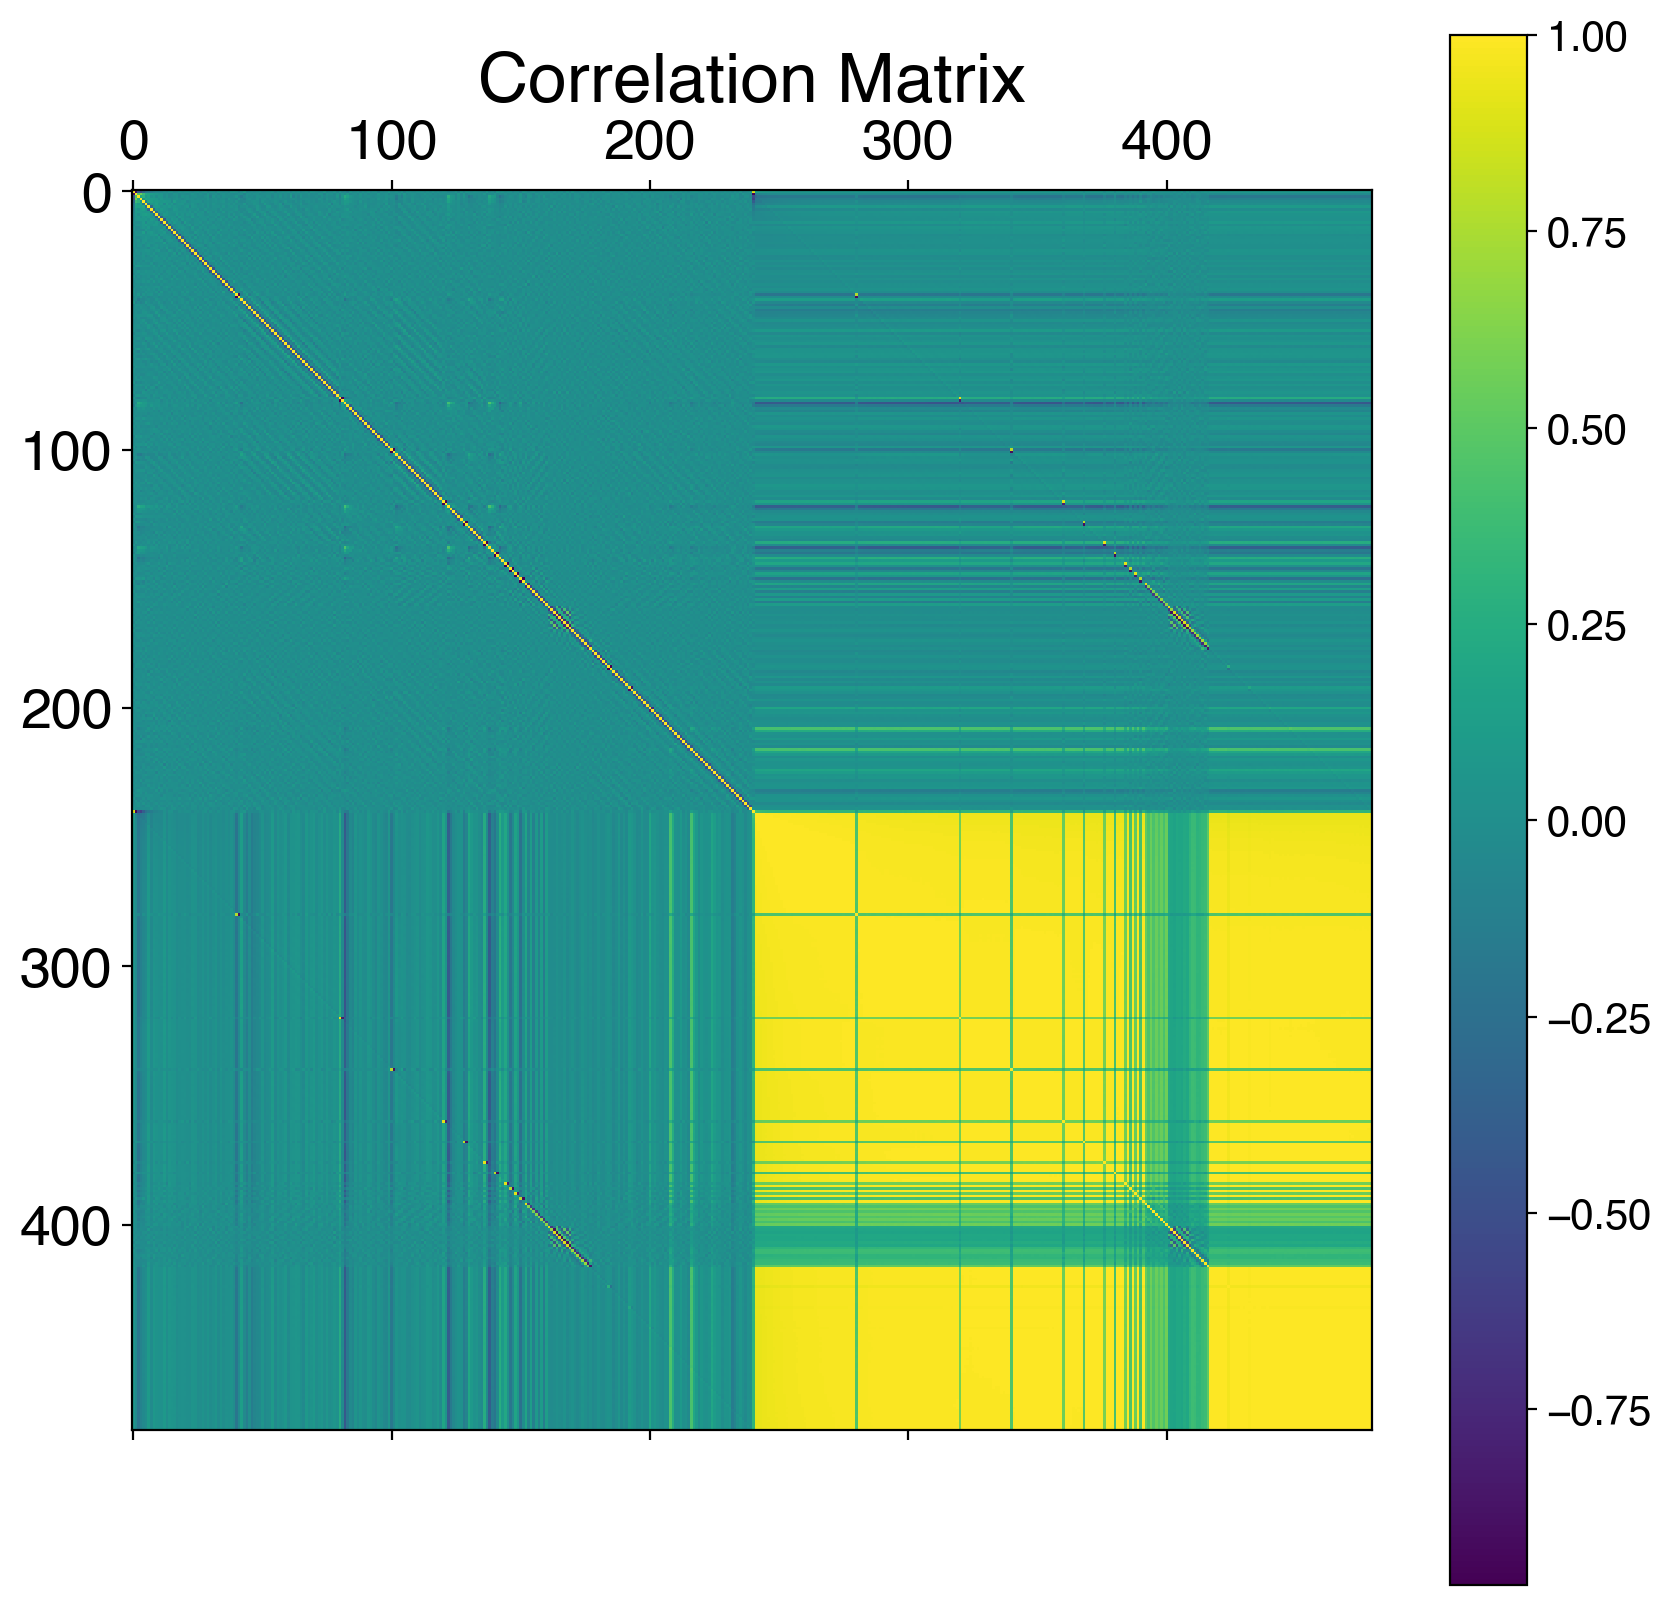
\includegraphics[width=0.35\textwidth]{../figures/correlation-matrix.png}
	\caption{Correlation matrix of features.}
	
	\label{fig:cor-mat}
\end{figure}

In Figure~\ref{fig:cor-mat}, the first, mainly green, quadrant correspond to slope features, while the fourth, mainly yellow, quadrant, averages.

\section{\acrlong{ols}}
\label{sec:results-ols}

As explained in Chapter~\ref{cha:methods}, \acrshort{ols} is treated here as a baseline. The actual vs. predicted plot in Figure~\ref{fig:ols-exposures} shows the predictions for unseen test data for both data sets.

\begin{figure}[!htb]
	\centering
	
	\begin{subfigure}[b]{1\textwidth}
		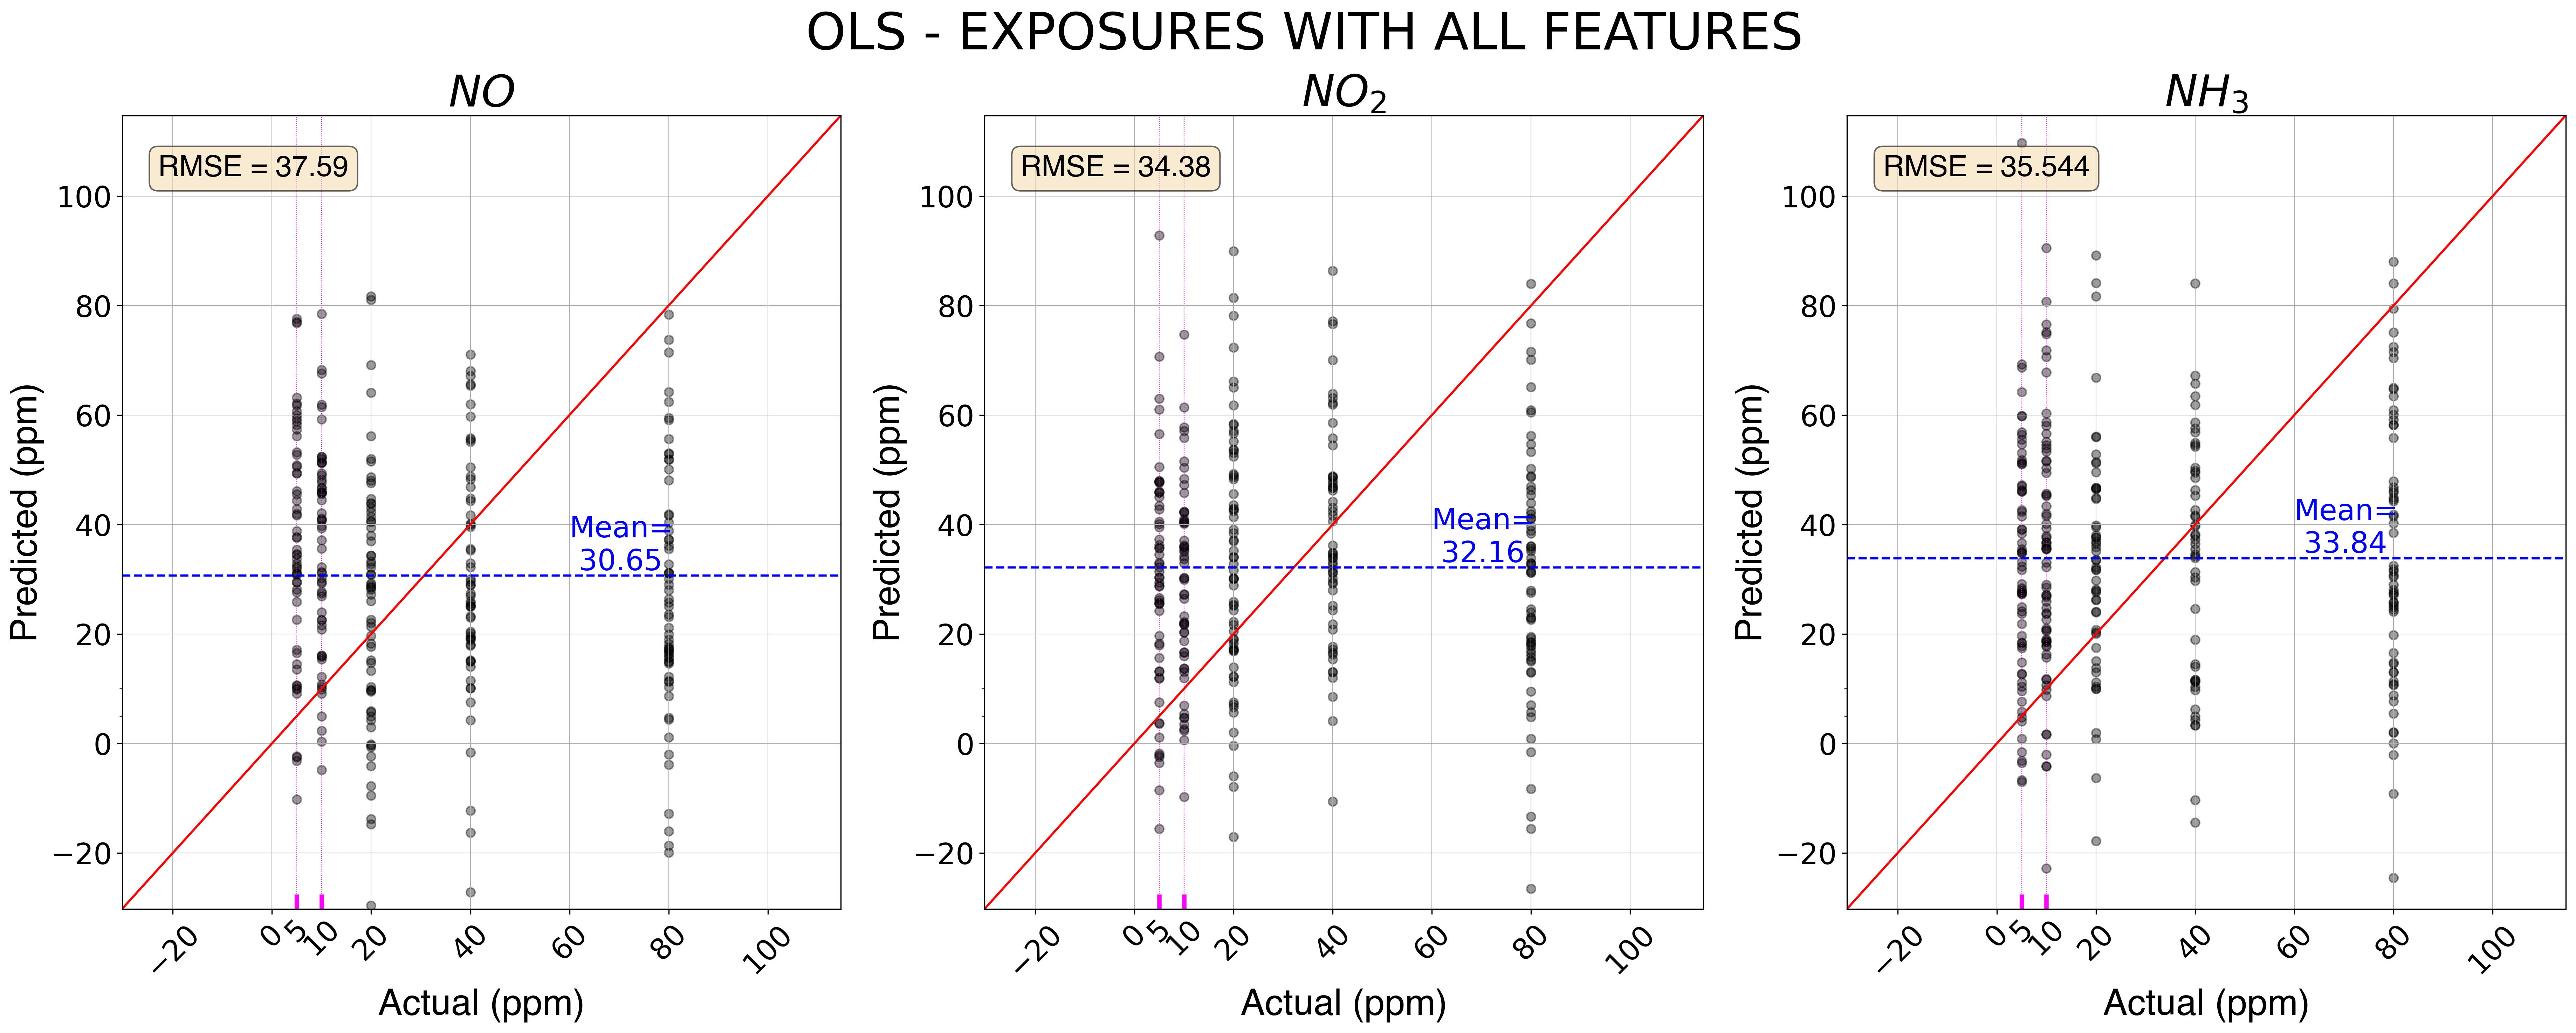
\includegraphics[width=1\linewidth]{../figures/ols-act-vs-pred.png}
		\caption{}
		\label{fig:ols-exposures} 
	\end{subfigure}
	
	\begin{subfigure}[b]{1\textwidth}
		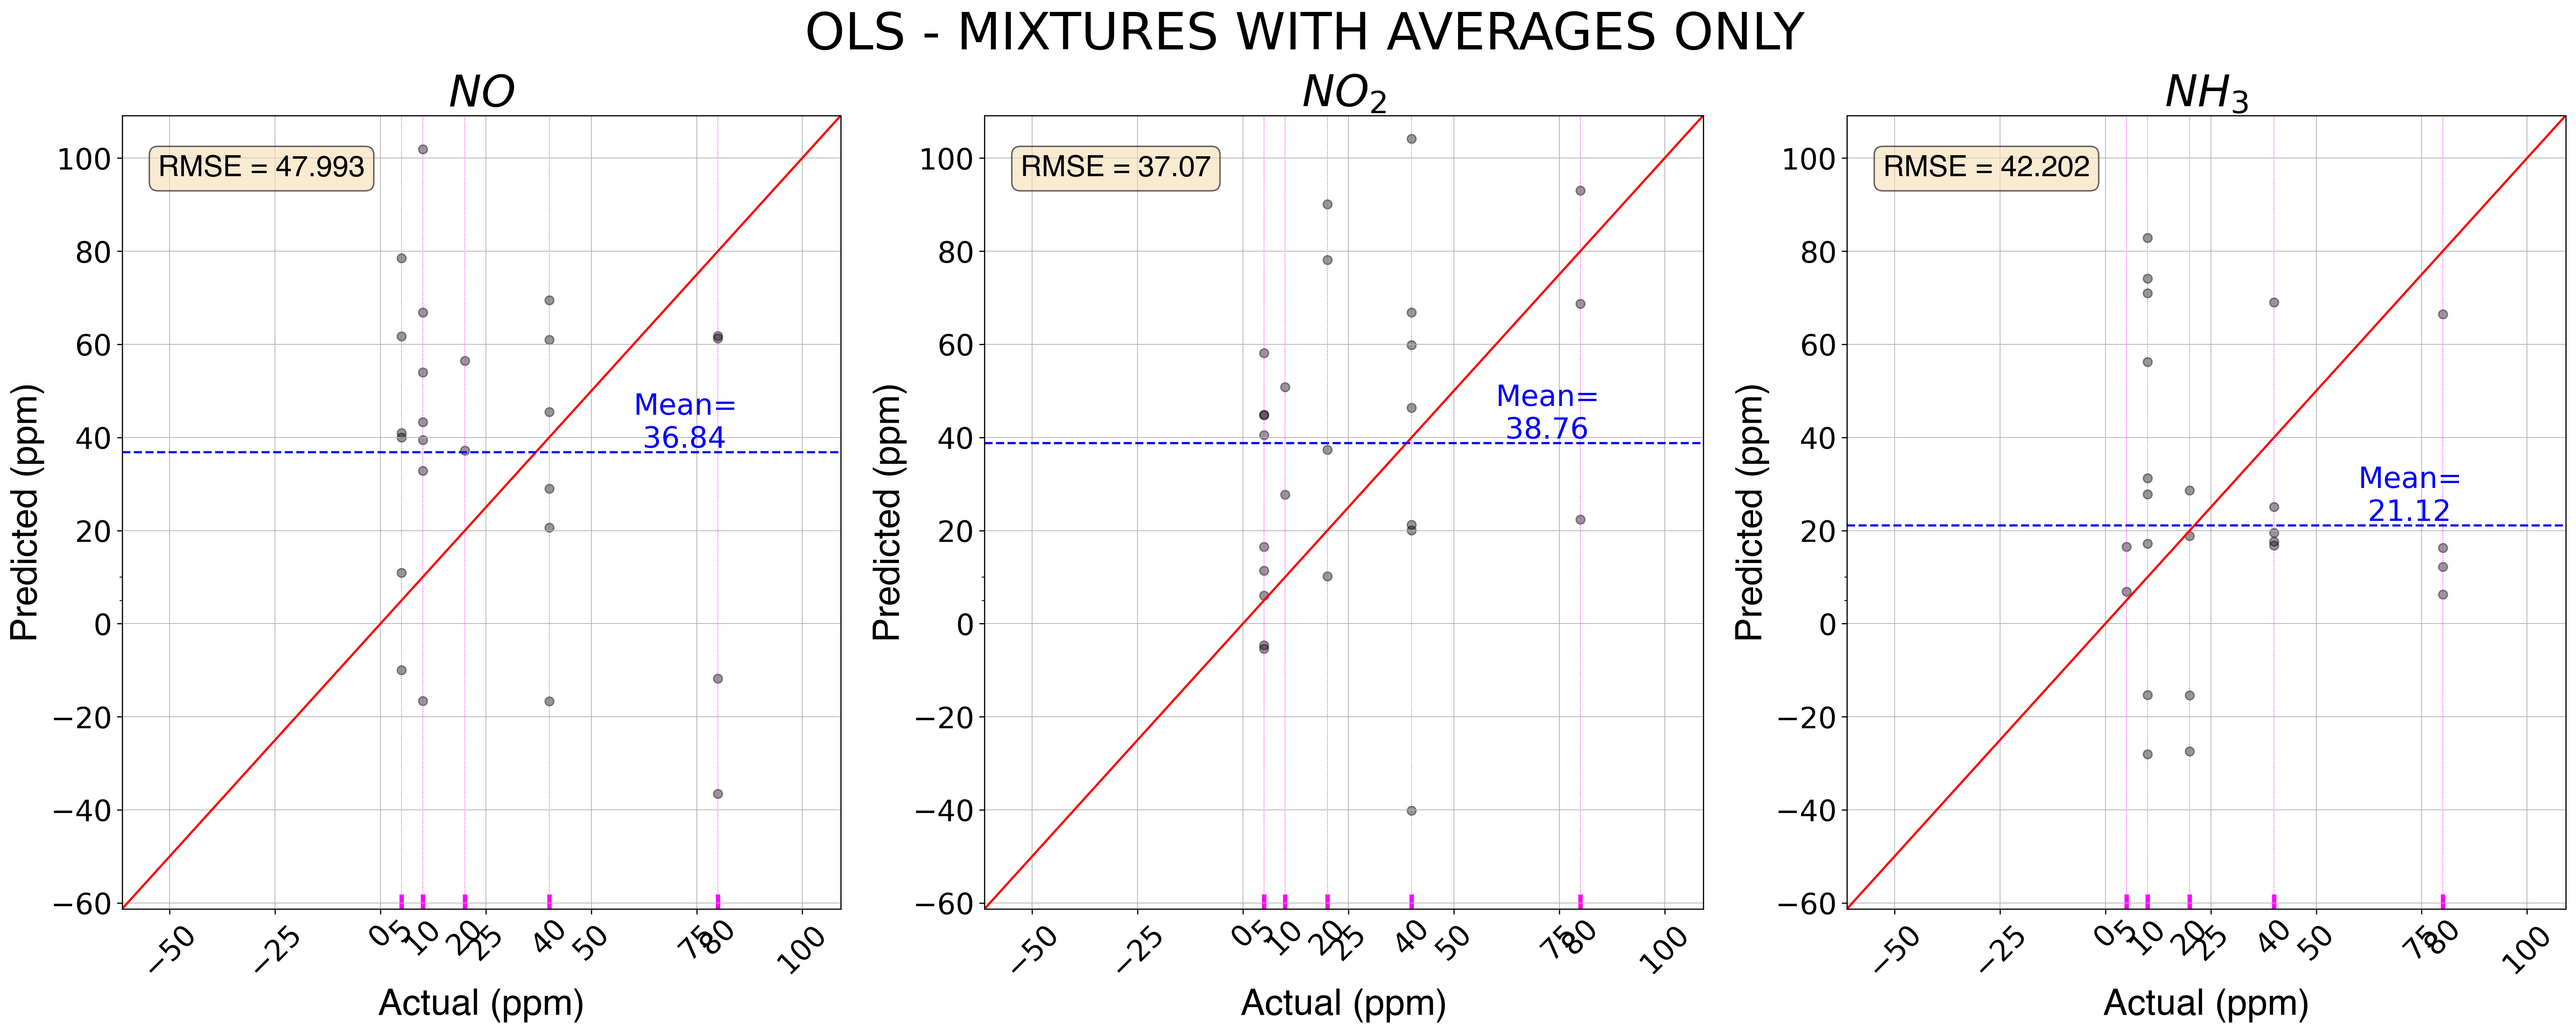
\includegraphics[width=1\linewidth]{../figures/ols-avg-act-vs-pred.png}
		\caption{}
		\label{fig:ols-averaged}
	\end{subfigure}
	
	\caption{Actual vs. Predicted for (a) slopes and averages through exposures and (b) only averaged average features through mixtures.}
	\label{fig:ols-both}
\end{figure}

Each subplot  in Figure~\ref{fig:ols-both} corresponds to predictions of \nox and ammonia concentrations, respectively. The red diagonal line is the  identity line. The blue line is the mean of predicted concentrations. The text box contains more information regarding the model fit, one being \acrshort{rmse}, which measures the error in the same scale as the targets, i.e. \acrshort{ppm} 

From Figure~\ref{fig:ols-both}, it can be seen that predictions are centered around the response mean for each gas, which is approximately 31\acrshort{ppm}. No prediction trend, however, is noticed, i.e. prediction concentrations have no relation with actual gas concentrations.

\section{\acrlong{pcr}}
\label{sec:results-pcr}

Following the methodology of Chapter~\ref{cha:methods}, a \acrshort{pca} is conducted with two components in an attempt to visualize the data in a lower-dimensional space in Figure~\ref{fig:pca-both}.  It is not possible to see any separation between the levels (i.e. concentrations) in both attempts.

\begin{figure}[!htb]
	\centering
	
	\begin{subfigure}[b]{1\textwidth}
	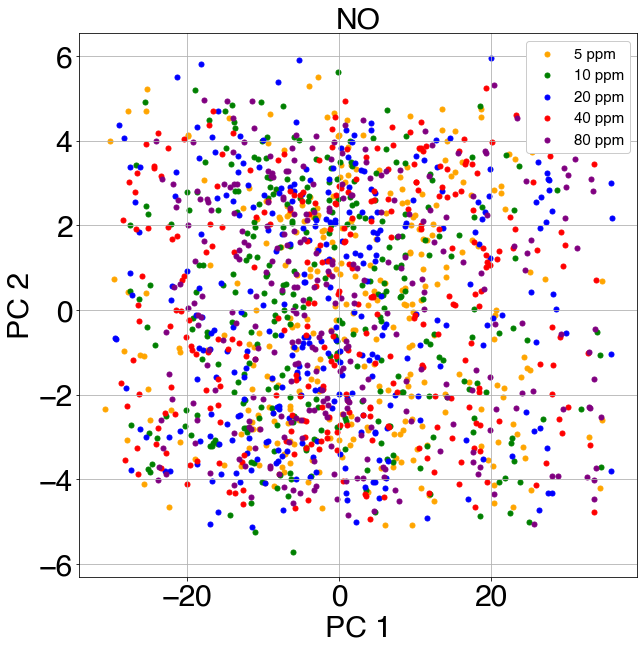
\includegraphics[width=0.30\textwidth]{../../figures/pcaNO.png}
	\hfill
	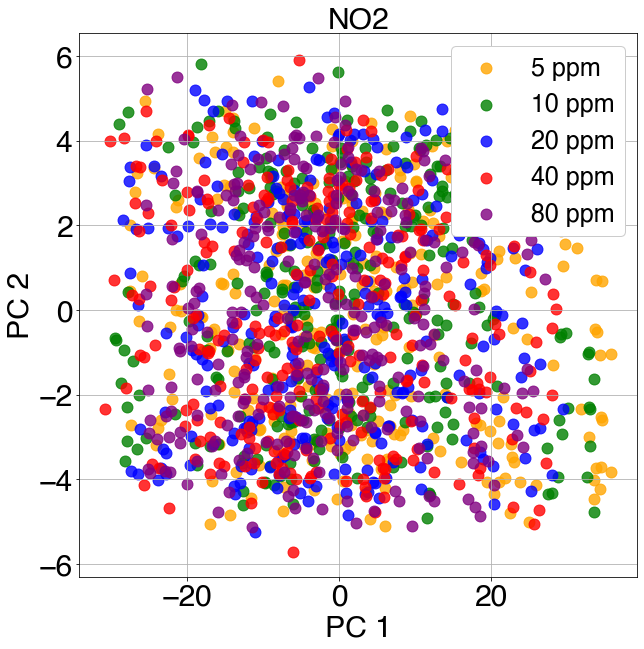
\includegraphics[width=0.30\textwidth]{../../figures/pcaNO2.png}
	\hfill
	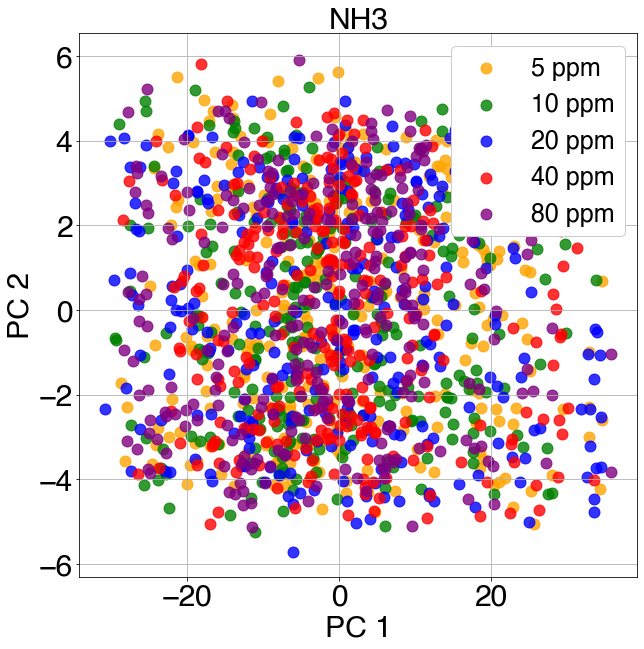
\includegraphics[width=0.30\textwidth]{../../figures/pcaNH3.png}
	\caption{}
	\label{fig:pca}
	\end{subfigure}
	
	\begin{subfigure}[b]{1\textwidth}
	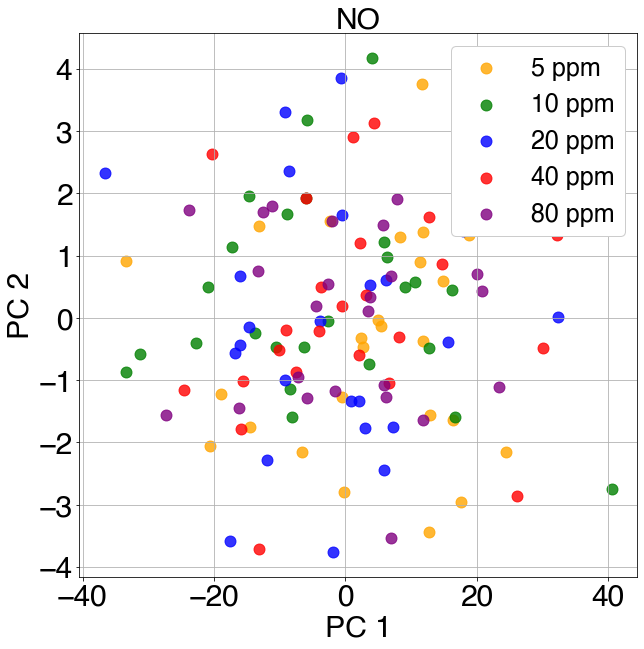
\includegraphics[width=0.30\textwidth]{../../figures/pcaNO-avg-feat.png}
	\hfill
	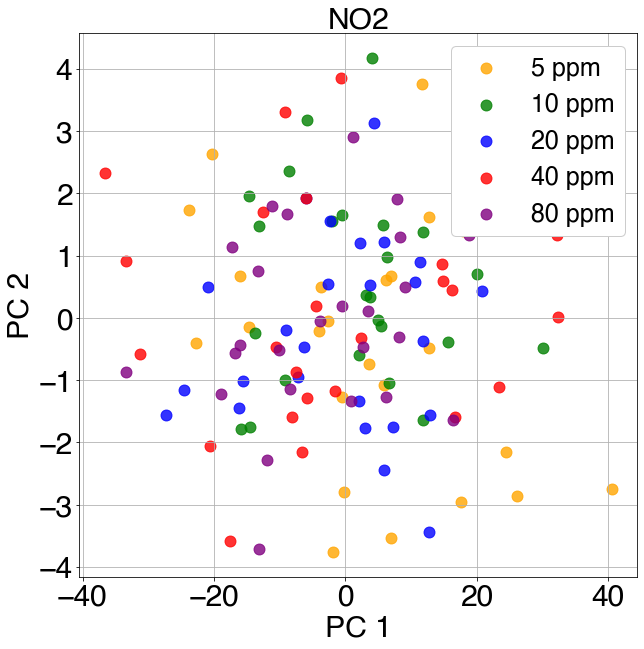
\includegraphics[width=0.30\textwidth]{../../figures/pcaNO2-avg-feat.png}
	\hfill
	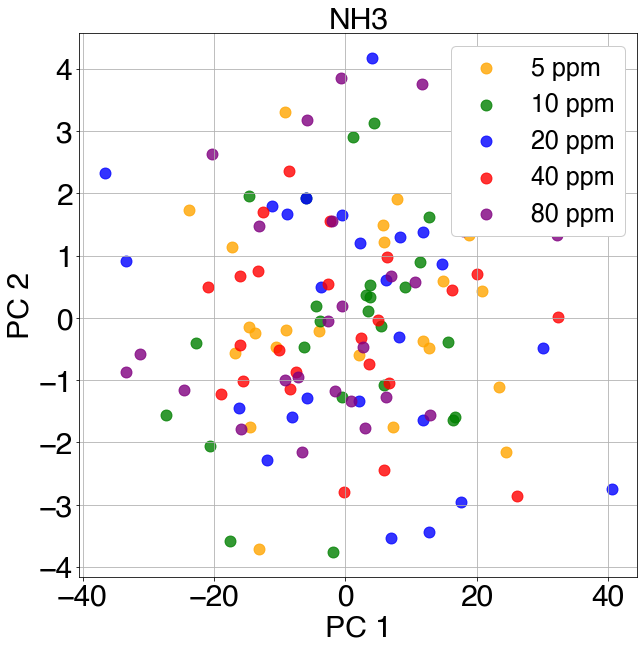
\includegraphics[width=0.30\textwidth]{../../figures/pcaNH3-avg-feat.png}
	\caption{}
	\label{fig:pca-avg-only}
	\end{subfigure}
	
	\caption{\acrshort{pca} for (a) slopes and averages through exposures and (b) only averaged average features through mixtures.}
	\label{fig:pca-both}
\end{figure}

Furthermore, an explained variance plot is shown in Figure~\ref{fig:pca-exp-var-both}. For the first case, the first two \acrshort{pc}s explain approximately 40\% of the total variance, reaching 80\% around 100 components. On the other hand, the second case achieves 90\% of explained variability with two components.

\begin{figure}[!htb]
	\centering

	\begin{subfigure}[t]{0.5\textwidth}
		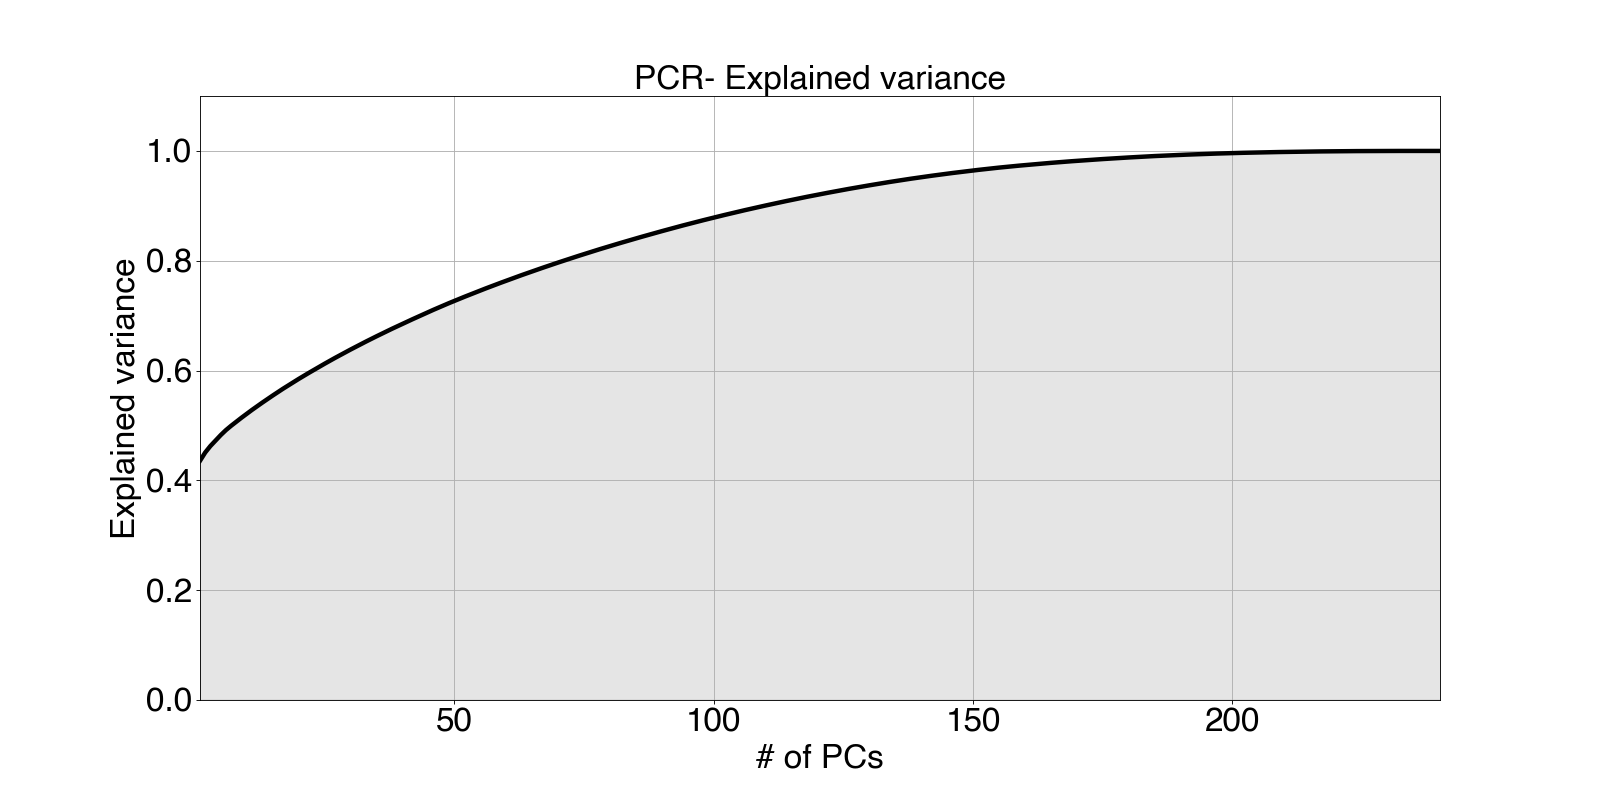
\includegraphics[width=1\linewidth]{../figures/pcr-explained-variance.png}
		\caption{}
		\label{fig:pca-exp-var} 
	\end{subfigure}
	
	\begin{subfigure}[t]{0.5\textwidth}
		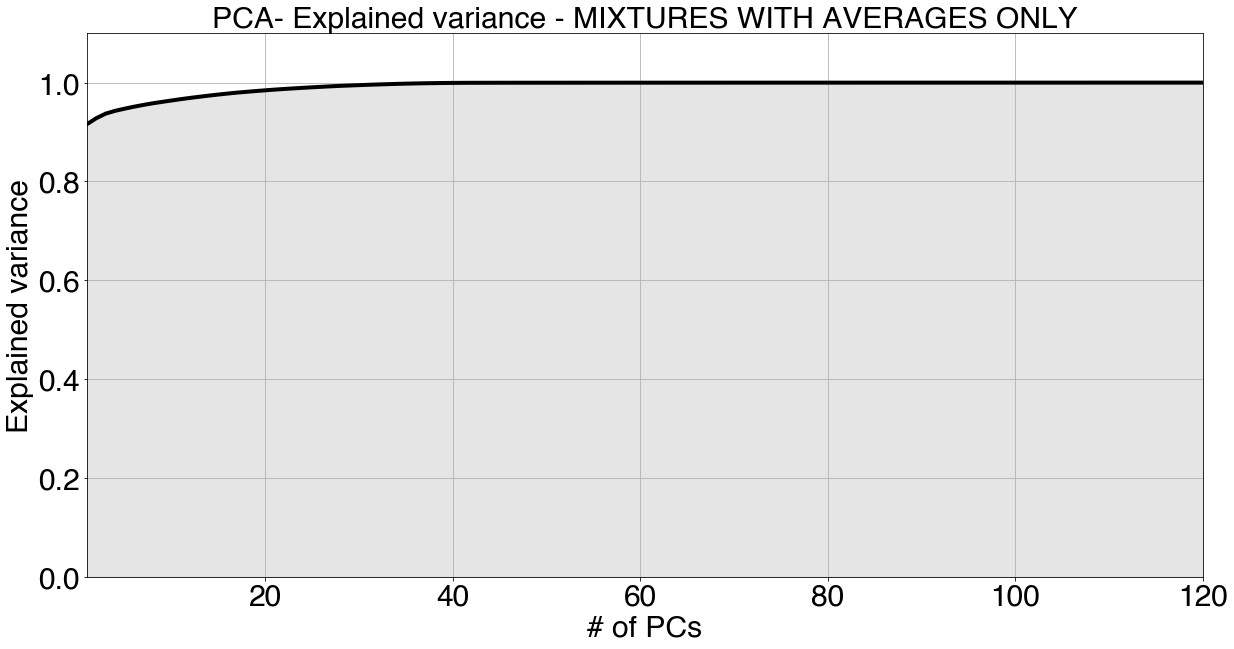
\includegraphics[width=1\linewidth]{../figures/pcr-explained-variance-avg-feat.png}
		\caption{}
		\label{fig:pca-exp-var-averaged}
	\end{subfigure}
	
	\caption{Explained variance of \acrshort{pc} for (a) slopes and averages through exposures and (b) only averaged average features through mixtures.}
	\label{fig:pca-exp-var-both}
\end{figure}

After this exploration of \acrshort{pca}, the analysis proceeds to fit a \acrshort{pcr} model to the data. The choice of number of \acrshort{pc}s was made via cross-validation using \acrshort{rmse} as the loss function, as can be seen in Figure~\ref{fig:pcr-cv-both}. Choosing only one component yields the minimum loss for both cases, around 27.

\begin{figure}[!htb]
	\centering
	
	\begin{subfigure}[t]{0.5\textwidth}
		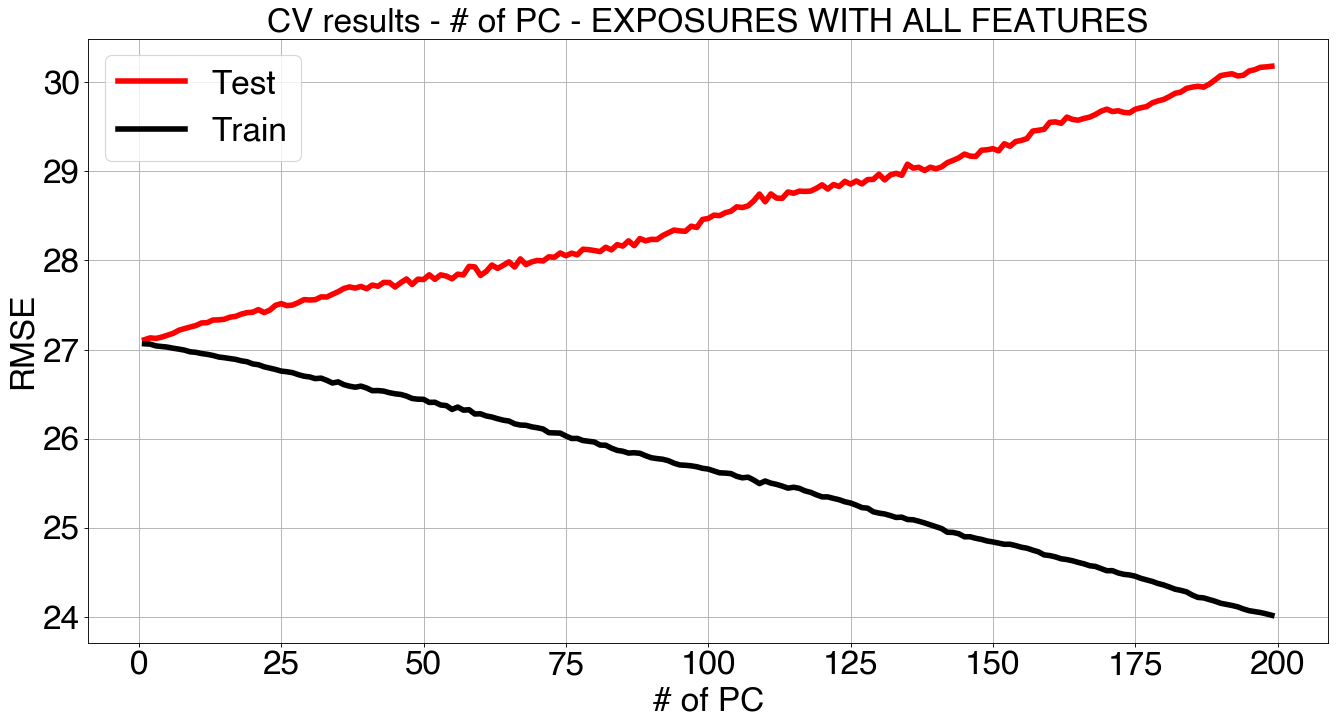
\includegraphics[width=1\linewidth]{../figures/pcr-cv.png}
		\caption{}
		\label{fig:pcr-cv} 
	\end{subfigure}
	
	\begin{subfigure}[t]{0.5\textwidth}
		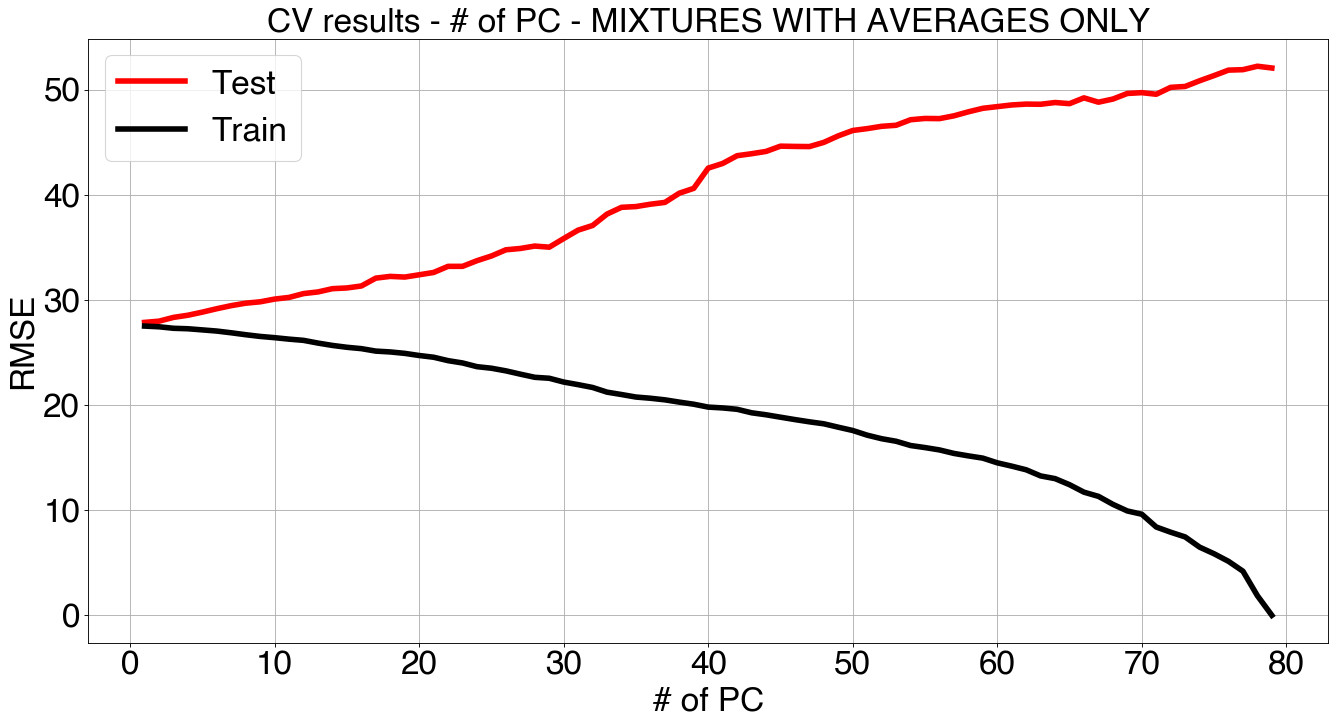
\includegraphics[width=1\linewidth]{../figures/pcr-cv-avg-feat.png}
		\caption{}
		\label{fig:pcr-cv-averaged}
	\end{subfigure}
	
	\caption{Cross-validation results for (a) slopes and averages through exposures and (b) only averaged average features through mixtures.}
	\label{fig:pcr-cv-both}
\end{figure}

After choosing the number of components, the regression was fit to the training data and used to predict with unseen test data. The results are shown in Figure~\ref{fig:pcr-both}. Once again, predicted concentrations are evenly spread around the mean.

\begin{figure}[!htb]
	\centering
	
	\begin{subfigure}[t]{1\textwidth}
		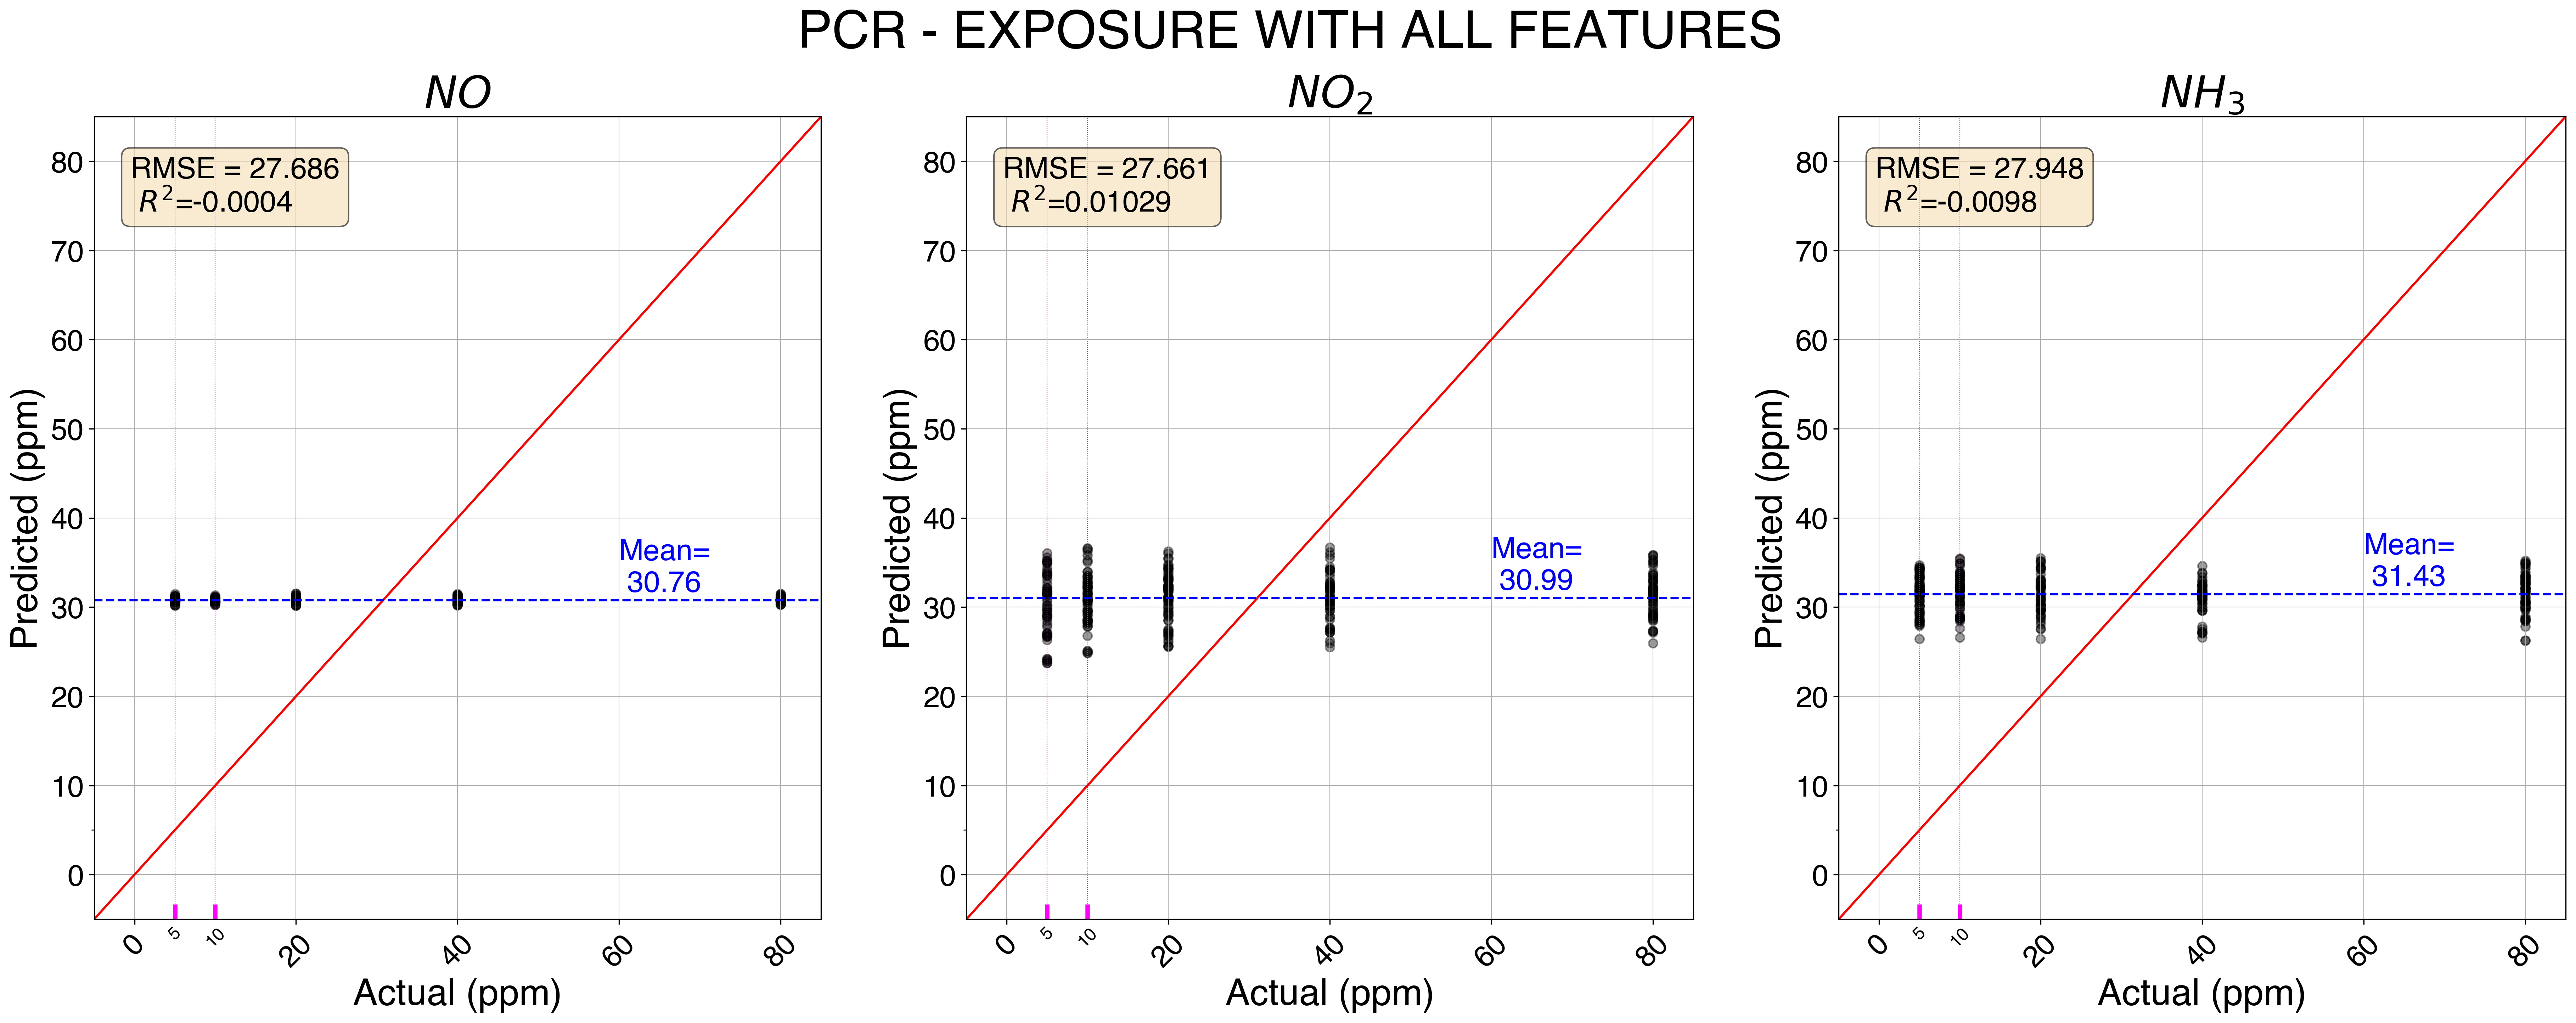
\includegraphics[width=1\linewidth]{../figures/pcr-act-vs-pred.png}
		\caption{}
		\label{fig:pcr-act-vs-pred} 
	\end{subfigure}
	
	\begin{subfigure}[t]{1\textwidth}
		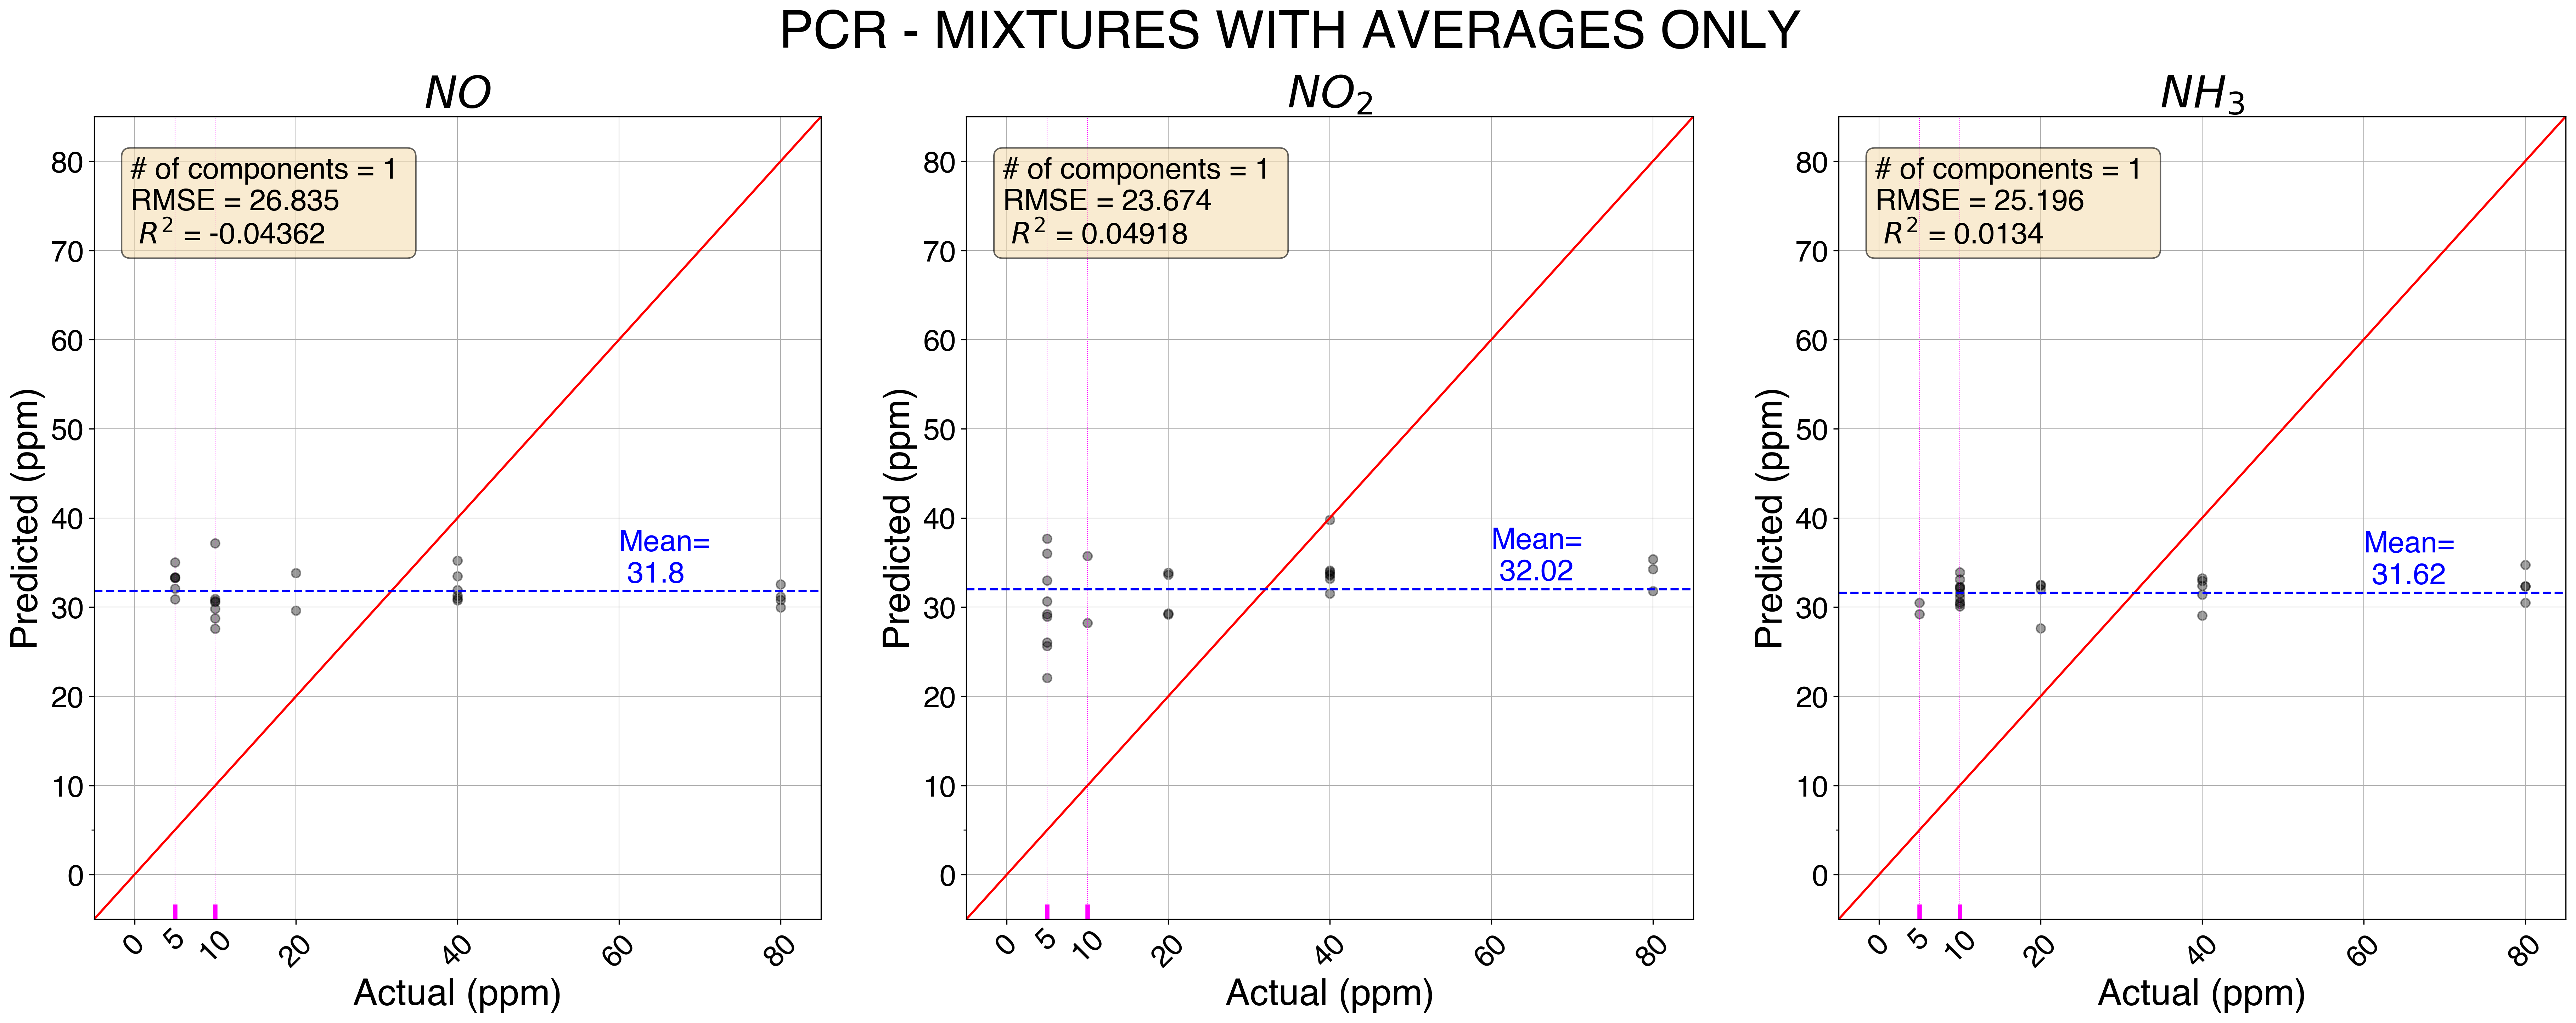
\includegraphics[width=1\linewidth]{../figures/pcr-act-vs-pred-avg-feat.png}
		\caption{}
		\label{fig:pcr-act-vs-pred-avg-feat}
	\end{subfigure}
	
	\caption{\acrshort{pcr} for (a) slopes and averages through exposures and (b) only averaged average features through mixtures.}
	\label{fig:pcr-both}
\end{figure}

\clearpage
\section{\acrlong{plsr}}
\label{sec:results-plsr}

Following the proposed model progression, the analysis proceeds to fit the \acrshort{plsr} model. A similar pipeline to Section~\ref{sec:results-pcr} was used. First, in Figure~\ref{fig:pls-both}, the choice of only two \acrshort{pls} components allowed visualization of data in a two-dimensional plot. Moreover, the total explained variance is shown in Figure~\ref{fig:pls-exp-var-both}. Once again, cross-validation using \acrshort{rmse} yields a single component as the best choice with an \acrshort{rmse} of approximately 27, which is then used to fit and predict  gas concentrations for unseen test data in Figure~\ref{fig:plsr-actual-vs-pred-both}.

\begin{figure}[!htb]
	\centering
	
	\begin{subfigure}[b]{1\textwidth}
		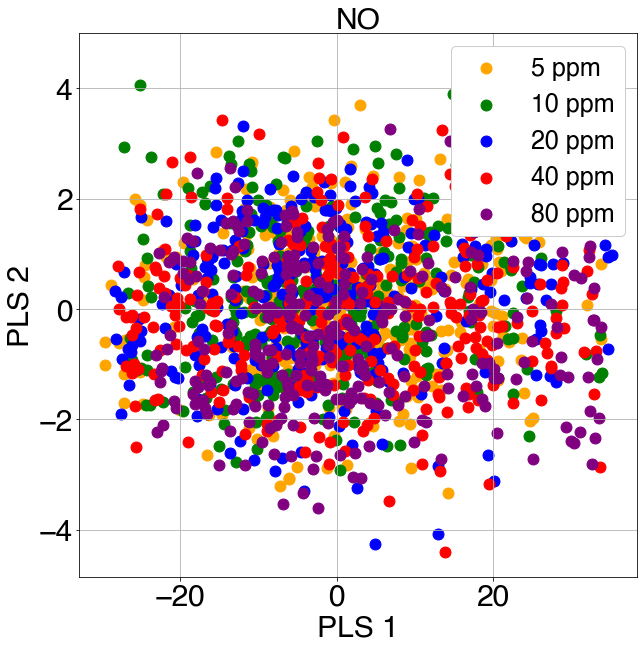
\includegraphics[width=0.30\textwidth]{../../figures/plsNO.png}
		\hfill
		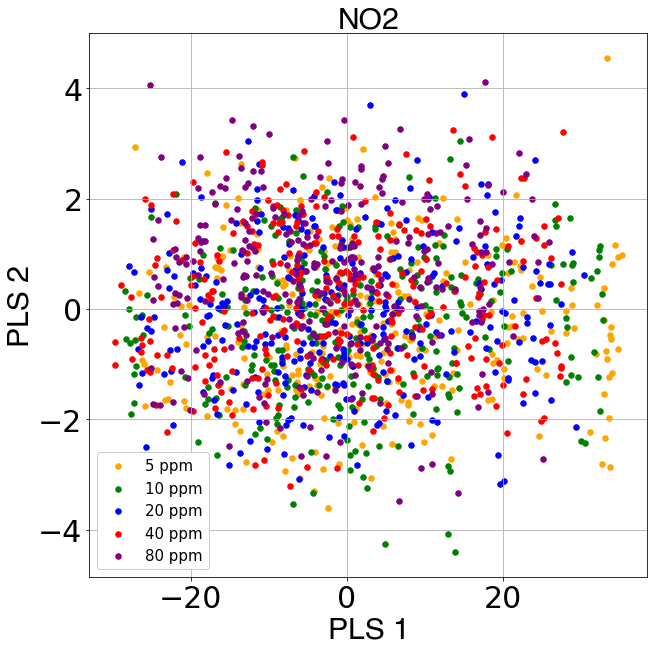
\includegraphics[width=0.30\textwidth]{../../figures/plsNO2.png}
		\hfill
		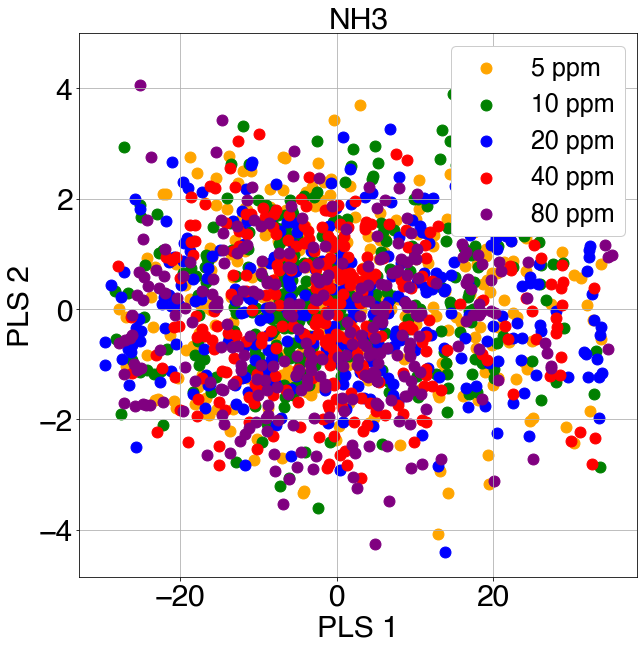
\includegraphics[width=0.30\textwidth]{../../figures/plsNH3.png}
		\caption{}
		\label{fig:pls}
	\end{subfigure}
	
	\begin{subfigure}[b]{1\textwidth}
		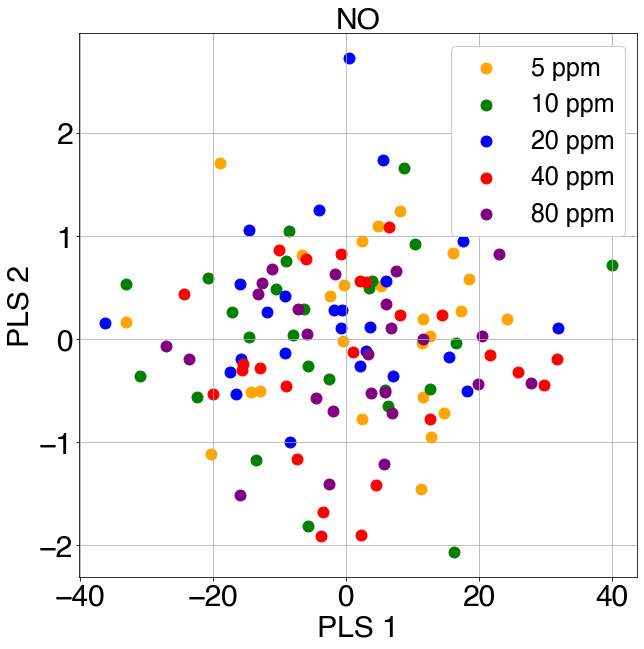
\includegraphics[width=0.30\textwidth]{../../figures/plsNO-avg-feat.png}
		\hfill
		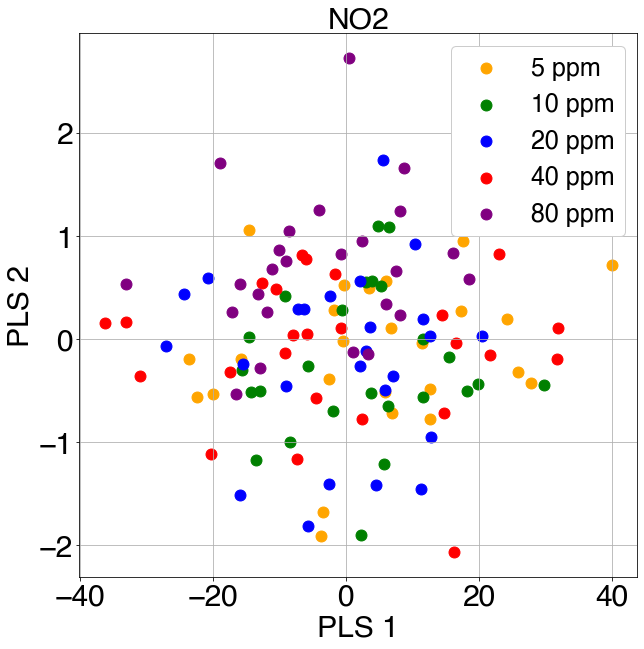
\includegraphics[width=0.30\textwidth]{../../figures/plsNO2-avg-feat.png}
		\hfill
		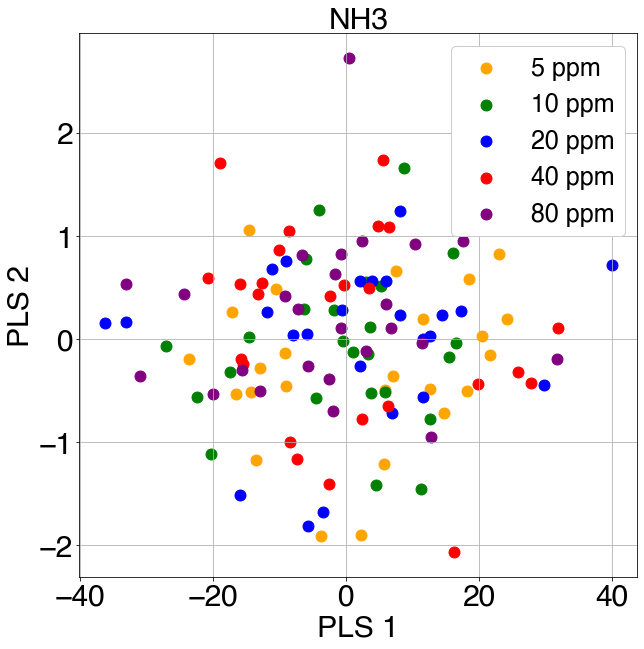
\includegraphics[width=0.30\textwidth]{../../figures/plsNH3-avg-feat.png}
		\caption{}
		\label{fig:pls-avg-only}
	\end{subfigure}
	
	\caption{\acrshort{pls} scores for (a) slopes and averages through exposures and (b) only averaged average features through mixtures.}
	\label{fig:pls-both}
\end{figure}

\begin{figure}[!htb]
	\centering
	
	\begin{subfigure}[t]{0.5\textwidth}
		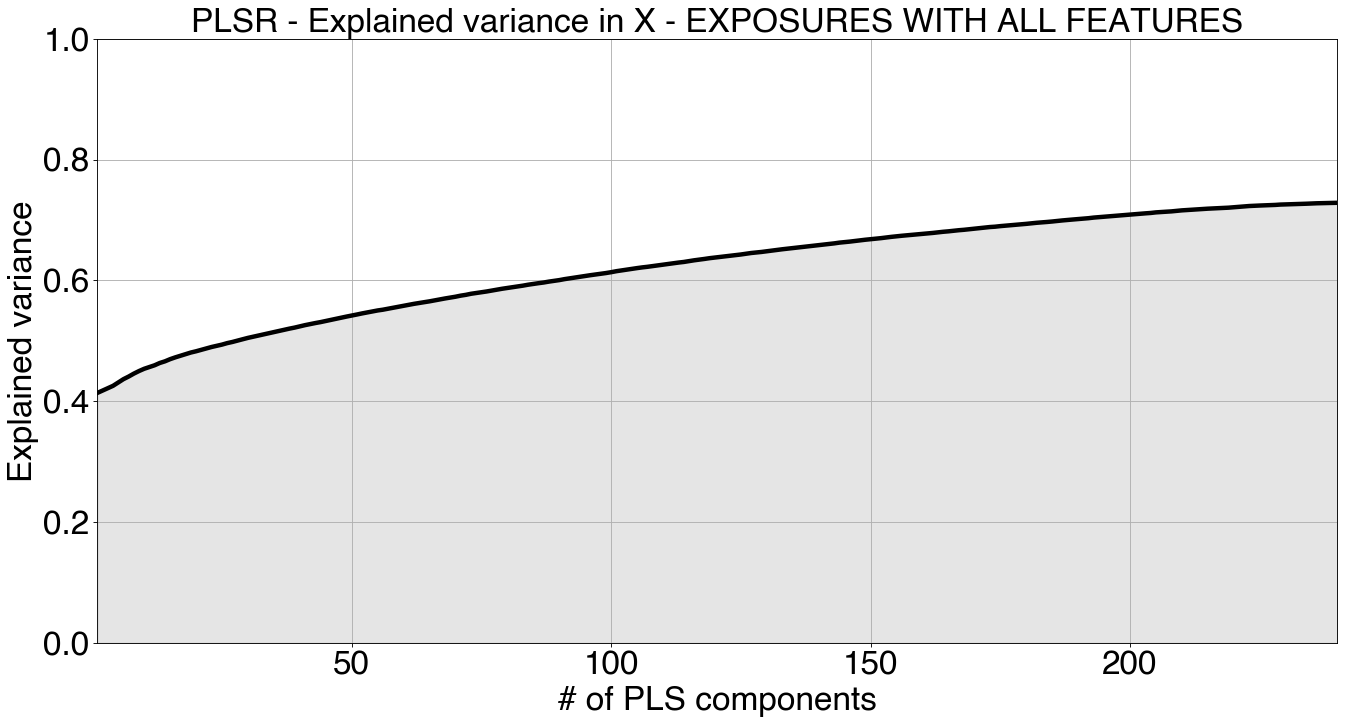
\includegraphics[width=1\linewidth]{../figures/pls-explained-variance.png}
		\caption{}
		\label{fig:pls-exp-var} 
	\end{subfigure}
	
	\begin{subfigure}[t]{0.5\textwidth}
		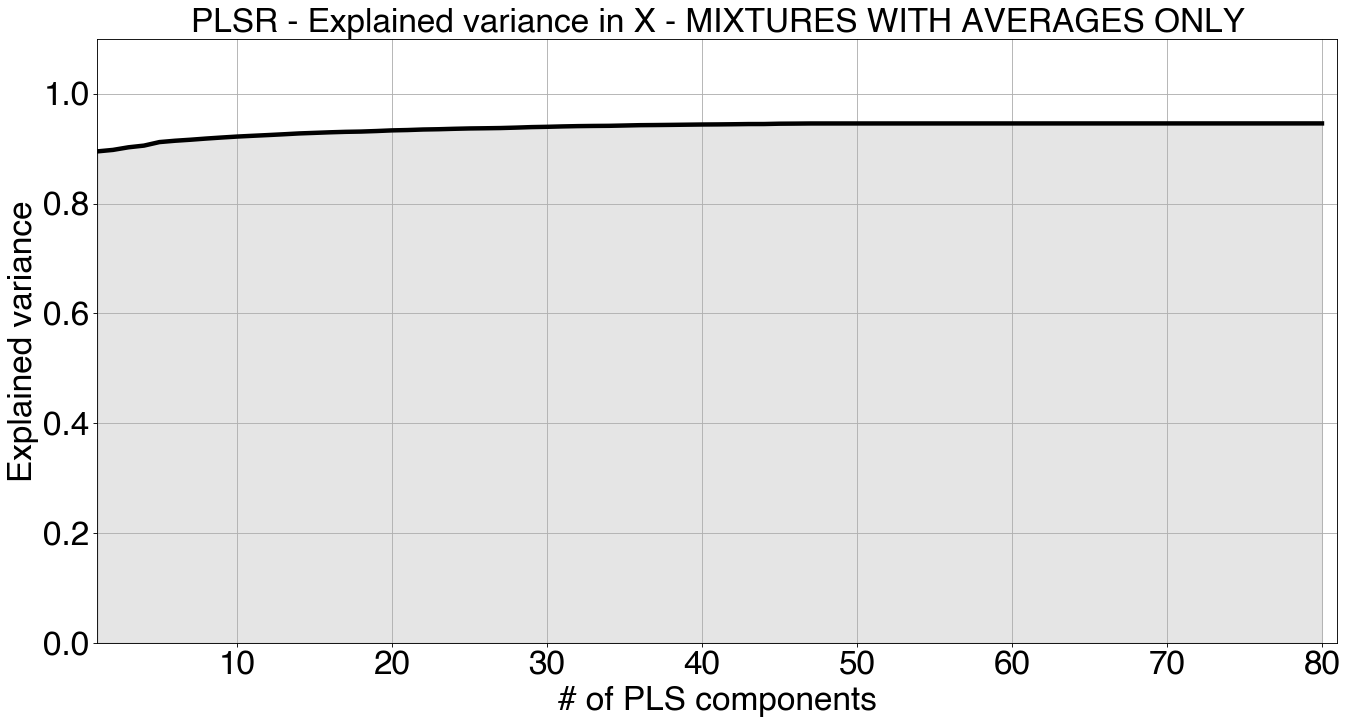
\includegraphics[width=1\linewidth]{../figures/pls-explained-variance-avg-feat.png}
		\caption{}
		\label{fig:pls-exp-var-avg-feat}
	\end{subfigure}
	
	\caption{Explained variance of \acrshort{pls} components for (a) slopes and averages through exposures and (b) only averaged average features through mixtures.}
	\label{fig:pls-exp-var-both}
\end{figure}


\begin{figure}[!htb]
	\centering
	
	\begin{subfigure}[t]{0.5\textwidth}
		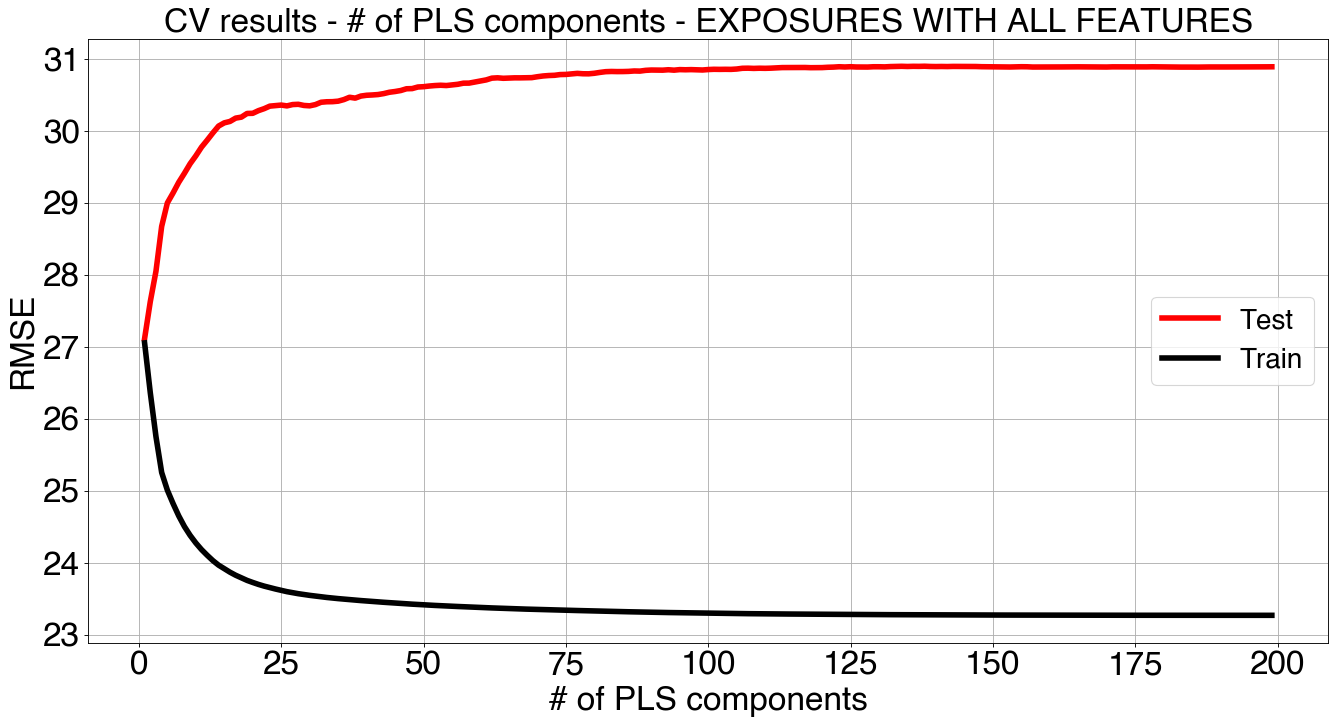
\includegraphics[width=1\linewidth]{../figures/pls-cv.png}
		\caption{}
		\label{fig:pls-cv} 
	\end{subfigure}
	
	\begin{subfigure}[t]{0.5\textwidth}
		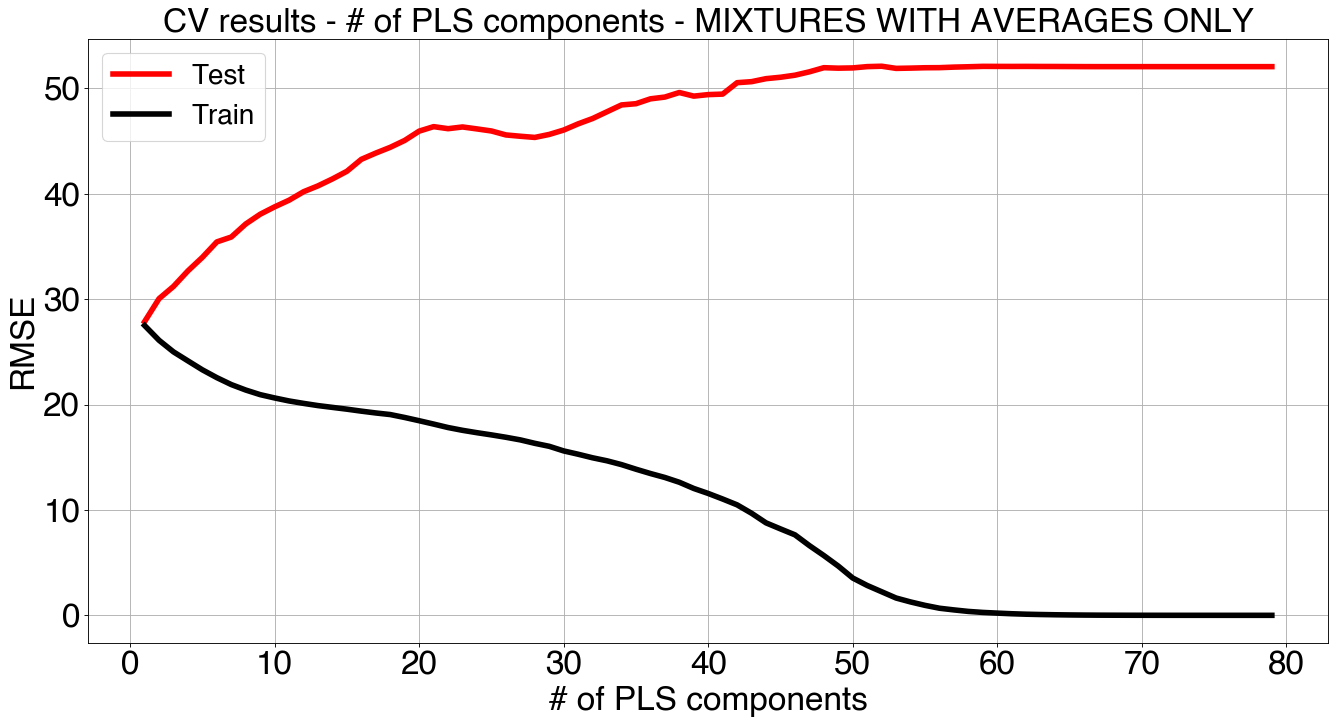
\includegraphics[width=1\linewidth]{../figures/pls-cv-avg-feat.png}
		\caption{}
		\label{fig:pls-cv-avg-feat}
	\end{subfigure}
	
	\caption{Cross-validation results for (a) slopes and averages through exposures and (b) only averaged average features through mixtures.}
	\label{fig:pls-cv-both}
\end{figure}

\begin{figure}[!htb]
	\centering
	
	\begin{subfigure}[t]{1\textwidth}
		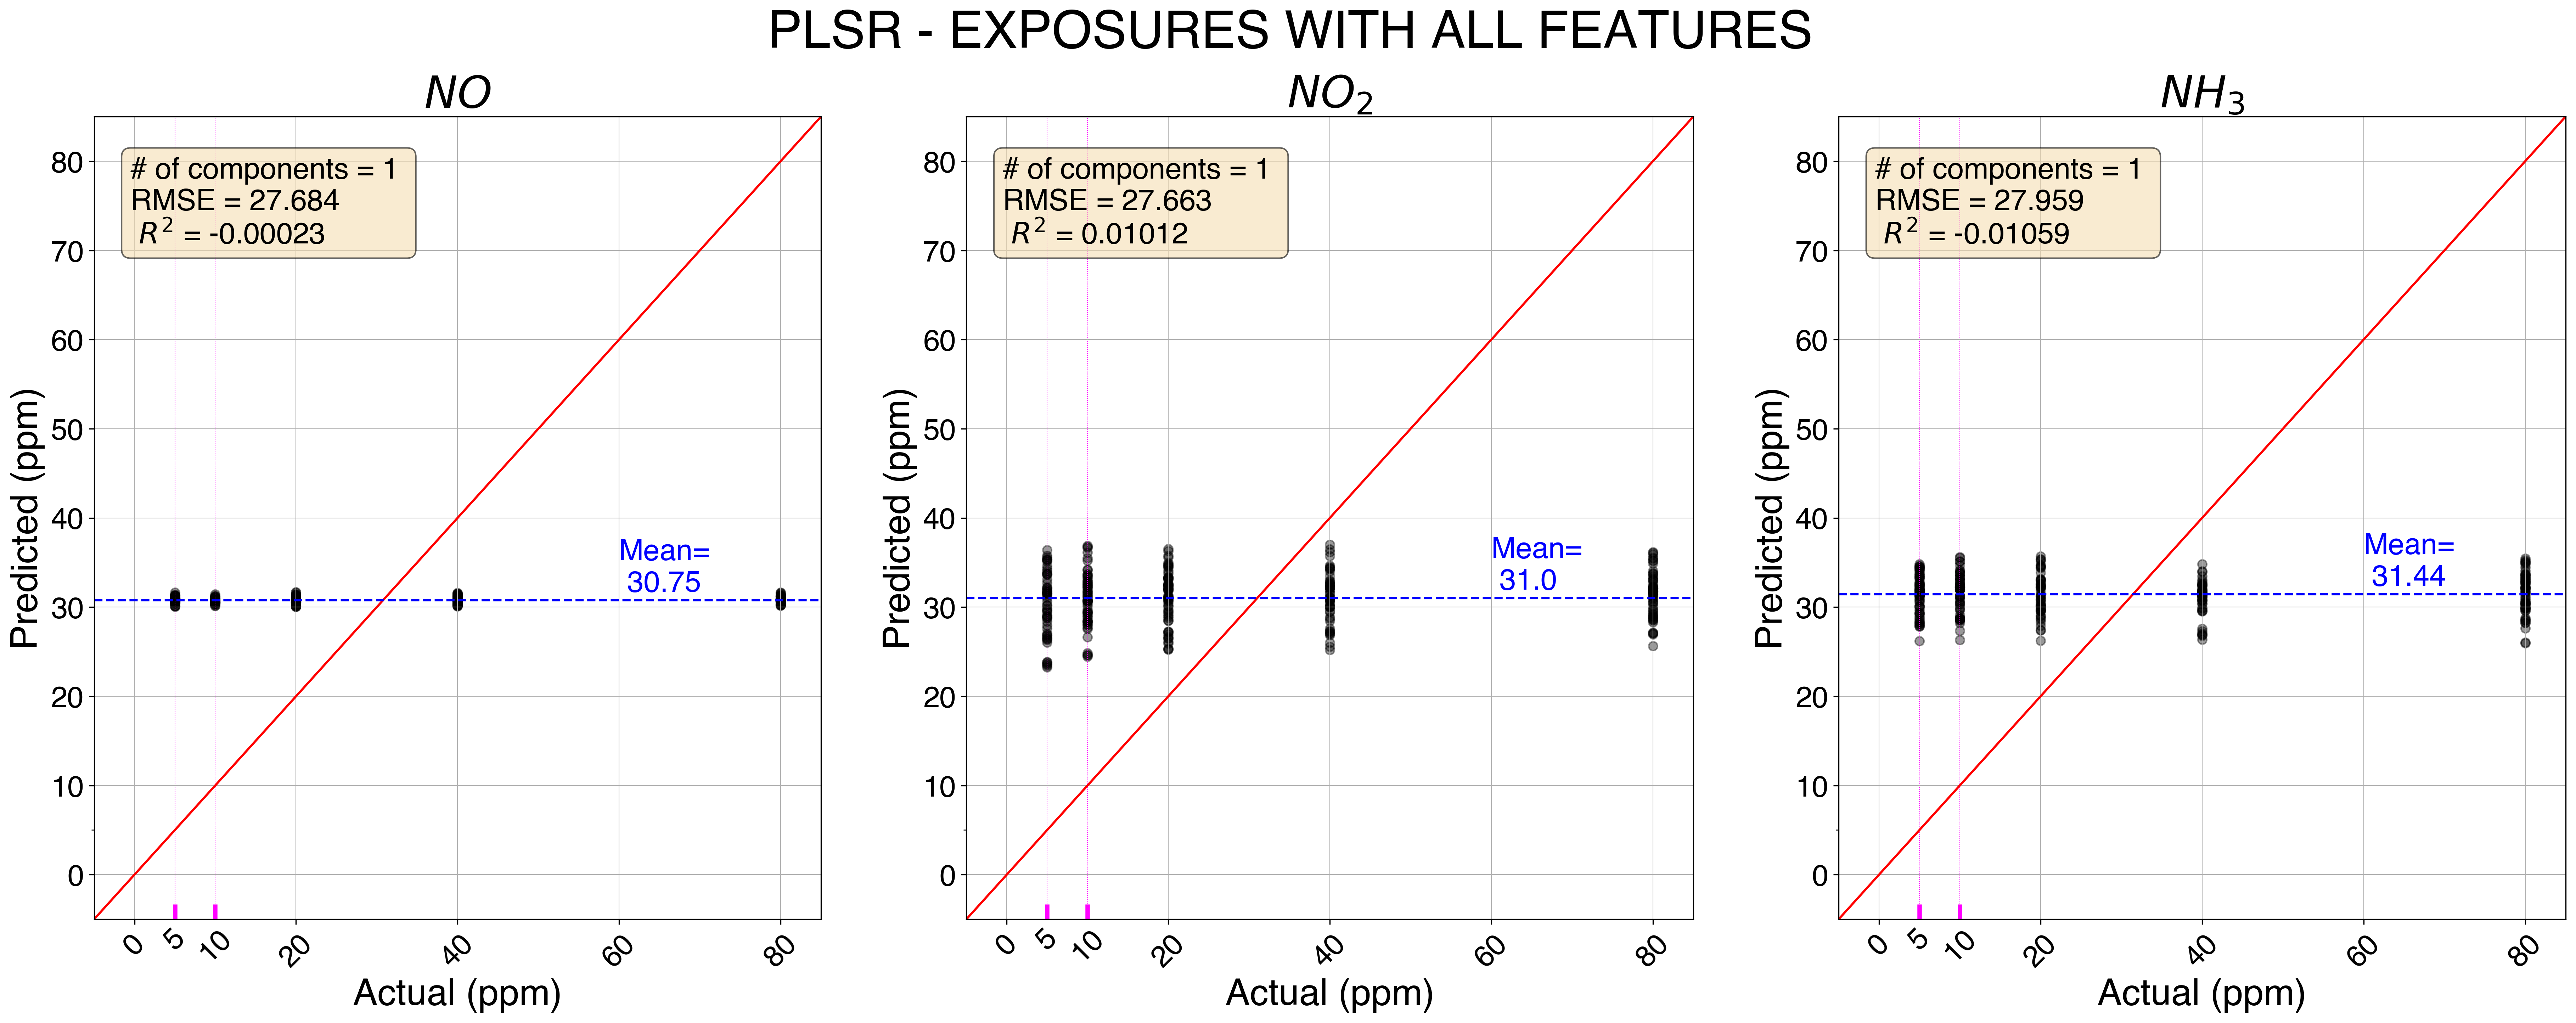
\includegraphics[width=1\linewidth]{../figures/plsr-act-vs-pred.png}
		\caption{}
		\label{fig:pls-act-vs-pred} 
	\end{subfigure}
	
	\begin{subfigure}[t]{1\textwidth}
		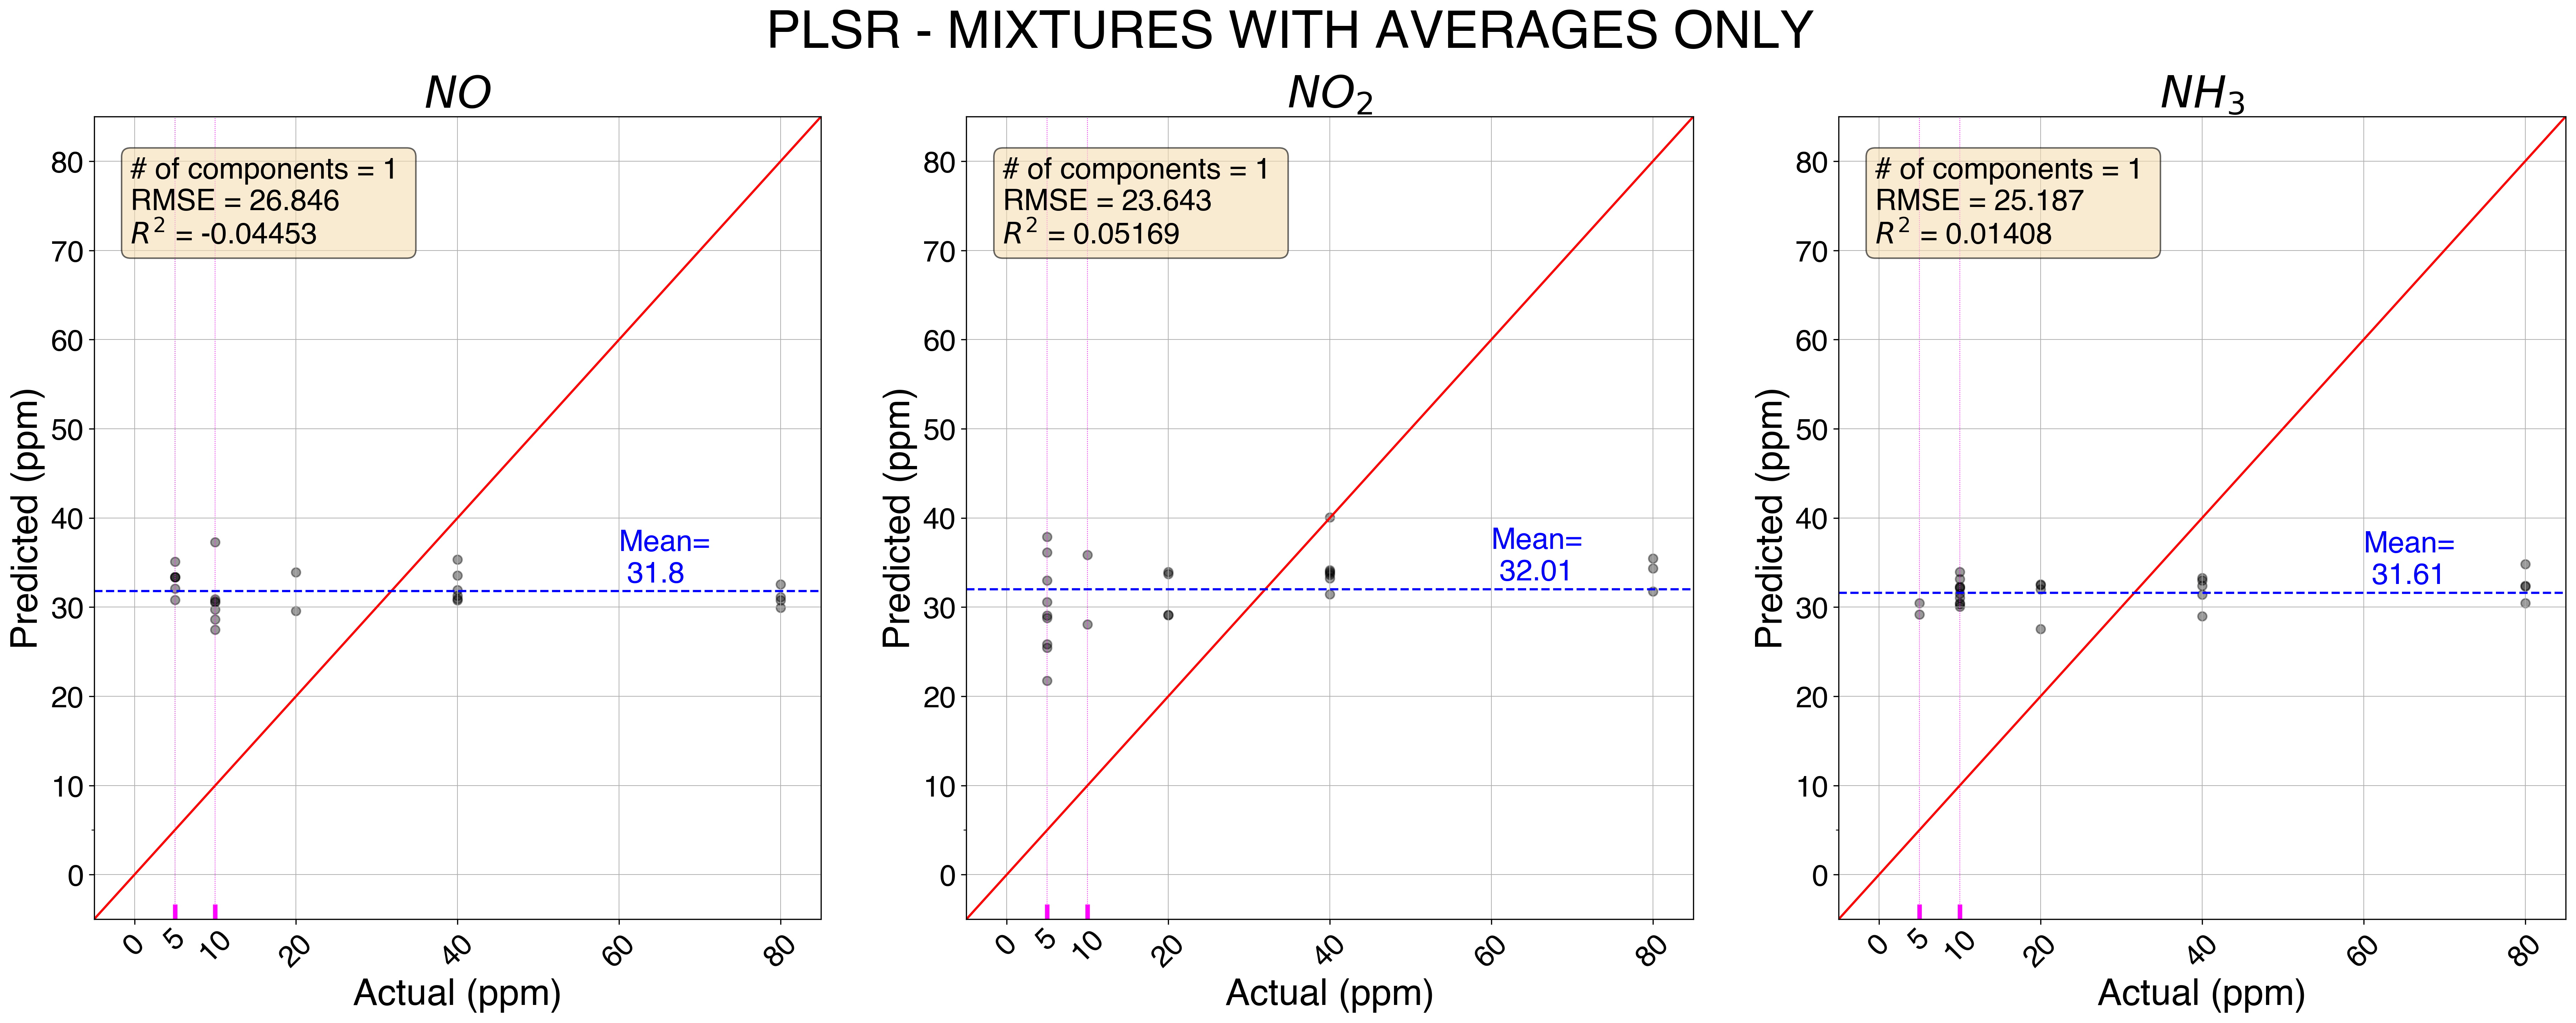
\includegraphics[width=1\linewidth]{../figures/plsr-act-vs-pred-avg-feat.png}
		\caption{}
		\label{fig:pls-act-vs-pred-avg-feat}
	\end{subfigure}
	
	\caption{\acrshort{plsr} for (a) slopes and averages through exposures and (b) only averaged average features through mixtures.}
	\label{fig:plsr-actual-vs-pred-both}
\end{figure}

The results here are similar to \acrshort{pcr}, with a significant smaller variance in predictions in comparison to \acrshort{ols} and equally spread around the blue lines, representing the target gas mean $\bar{y} \approx 31$ppm.

It is possible to gain more insight on the regression process by plotting the predictions for training data. For example, in Figure~\ref{fig:pls-cv}, the model with minimum training error is the one with 199 \acrshort{pls} components (although from approximately 125 components the \acrshort{rmse} is virtually constant around 23). Despite performing badly at unseen test data at this point, the training data predictions are shown in Figure~\ref{fig:plsr-TRAIN-PRED}. From it, it is possible to see some prediction trend and relatively higher values of $R^2$. However, predictions have high variance, and despite being a complex model regarding number of regressors, one cannot say it overfitted. The main idea here is to show that the model performs poorly even on training data. This behavior is seen again in other models, and similar plots as Figure~\ref{fig:plsr-TRAIN-PRED} are suppressed in favor of conciseness.

\begin{figure}[!h]
	\centering
	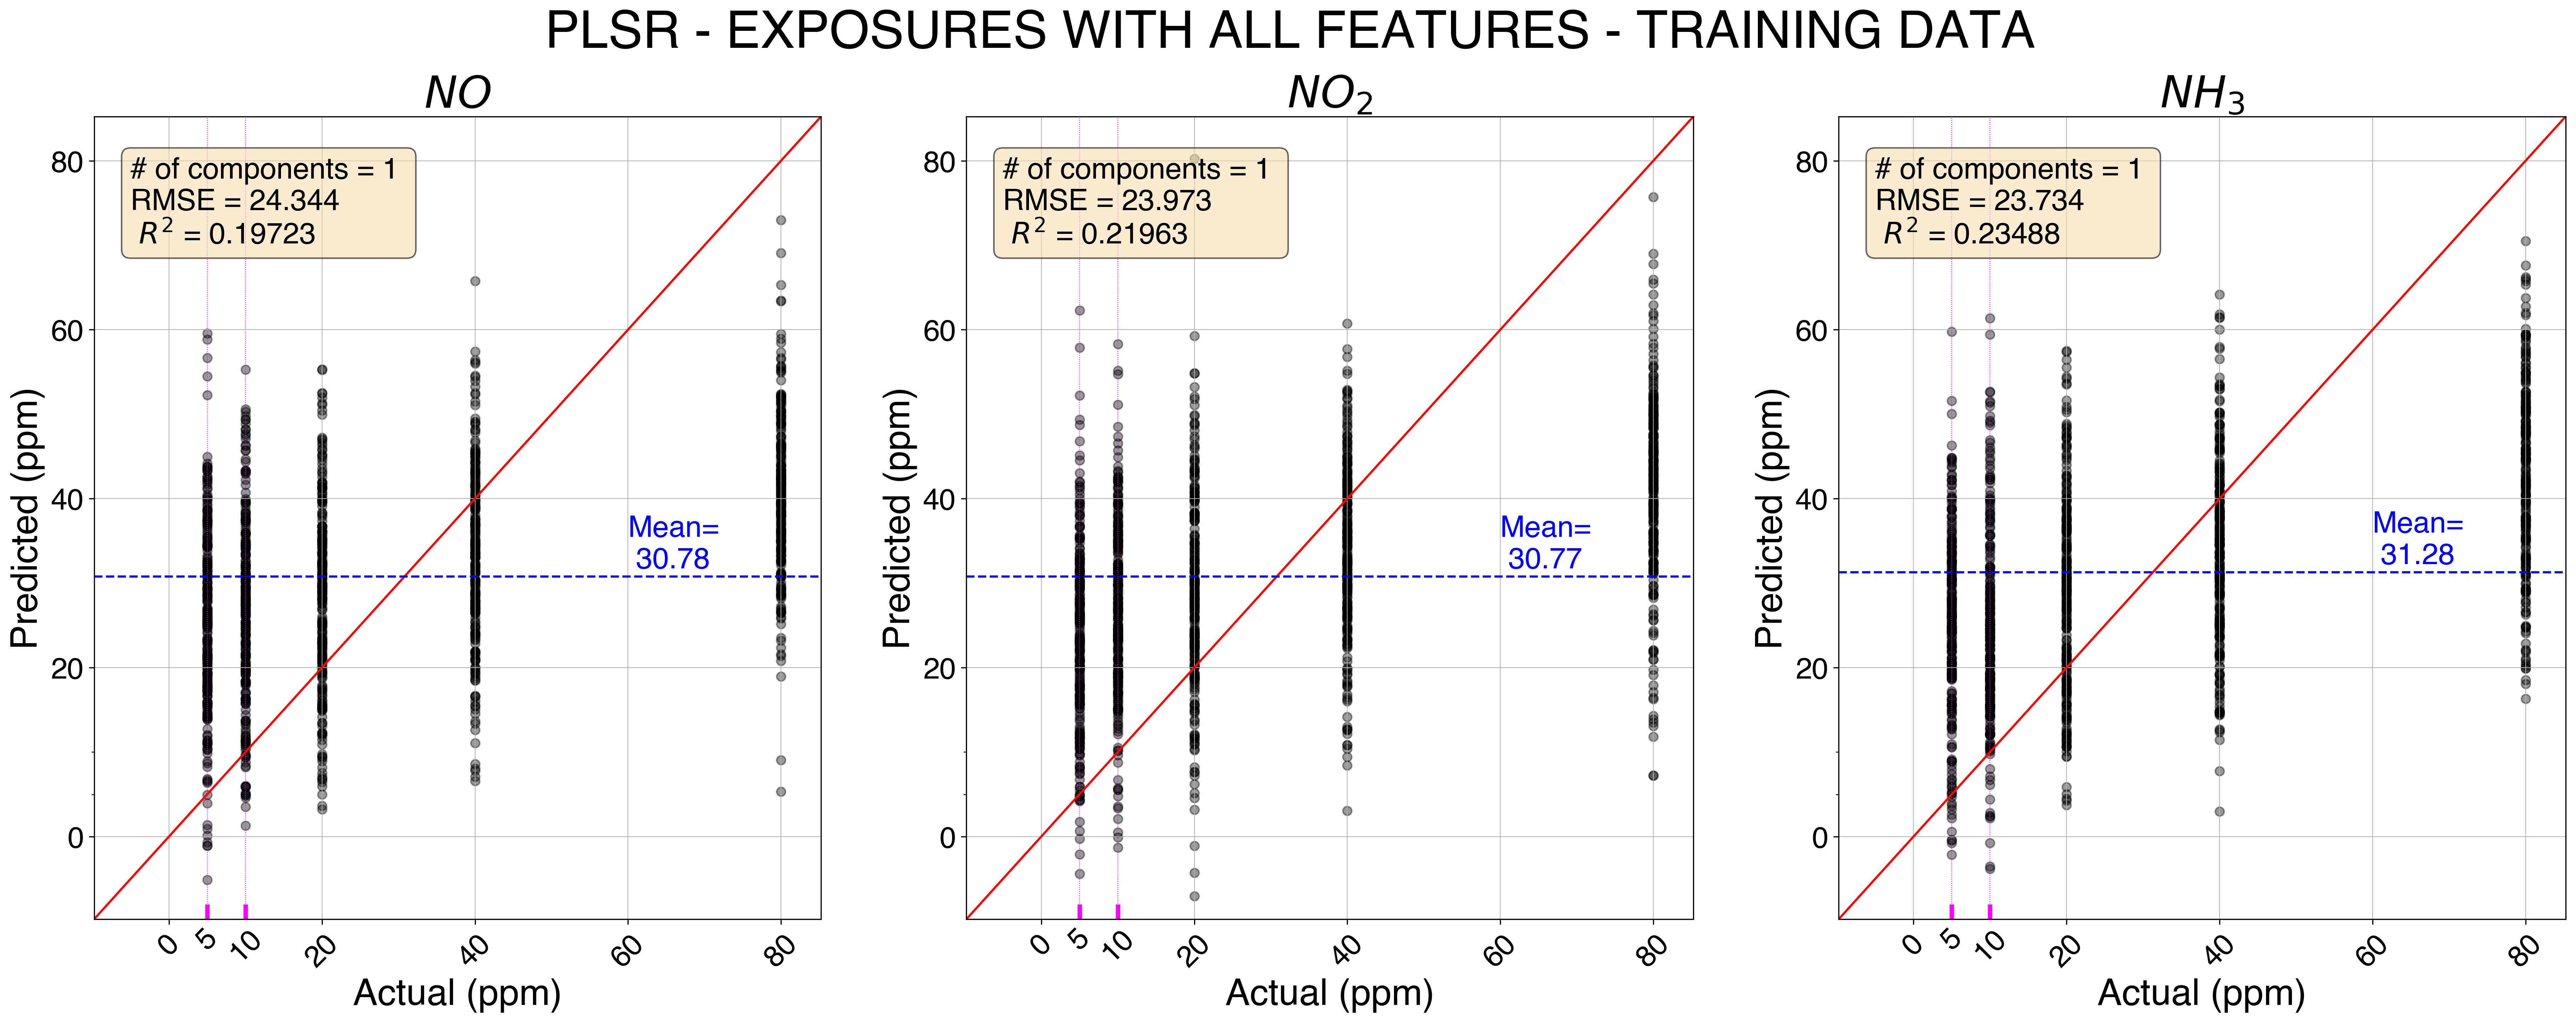
\includegraphics[width=1\textwidth]{../figures/PLSR-TRAINING-DATA.png}
	\caption{Prediction for training data using the \acrshort{plsr} model with minimal \acrshort{rmse}.}
	\label{fig:plsr-TRAIN-PRED}
\end{figure}


\clearpage
\section{Ridge Regression}
\label{sec:results-ridge}

For Ridge regression, the regularization term $\lambda$ was chosen via cross-validation, as shown in Figure~\ref{fig:ridge-cv-both}. Additionally, the shrinkage of coefficients can be seen in Figure~\ref{fig:ridge-shrink-both}. As expected, the coefficients shrink asymptotically towards zero.

\begin{figure}[!htb]
	\centering
	
	\begin{subfigure}[t]{0.6\textwidth}
		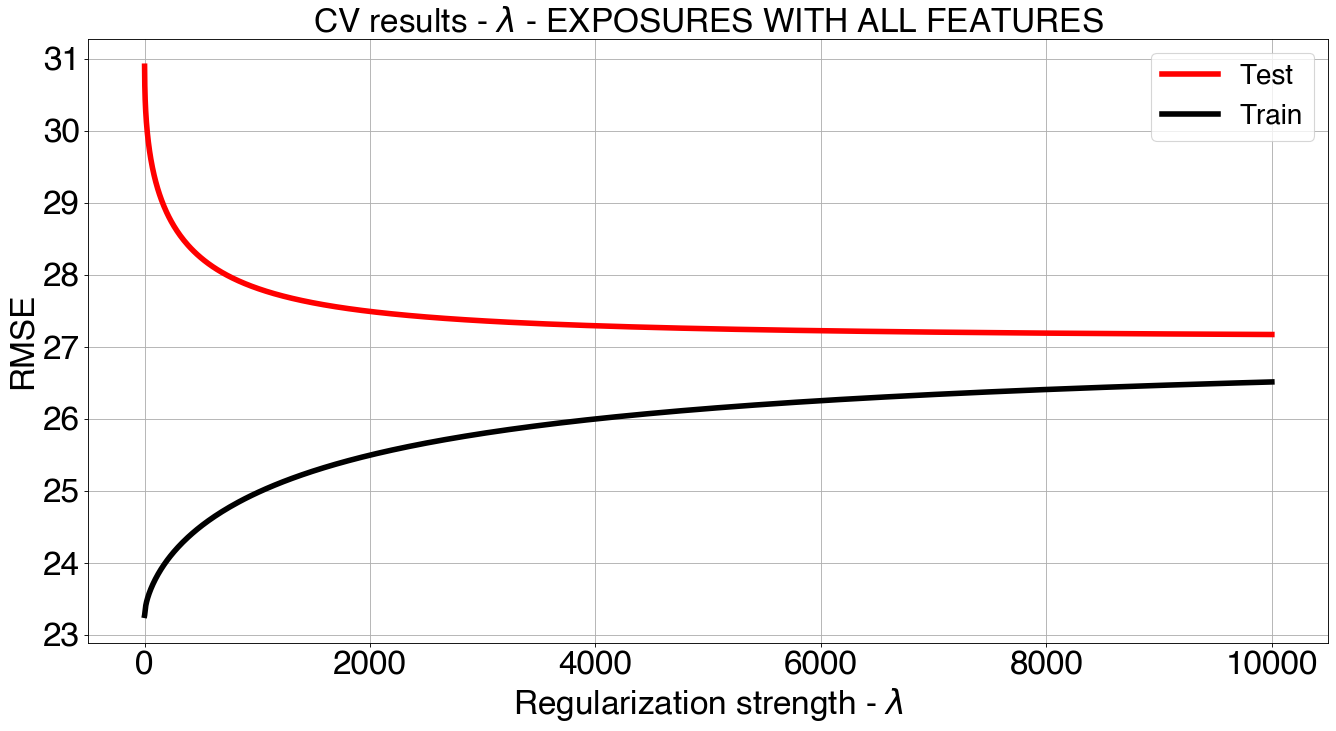
\includegraphics[width=1\linewidth]{../figures/ridge-cv.png}
		\caption{}
		\label{ridge:pls-cv} 
	\end{subfigure}
	
	\begin{subfigure}[t]{0.6\textwidth}
		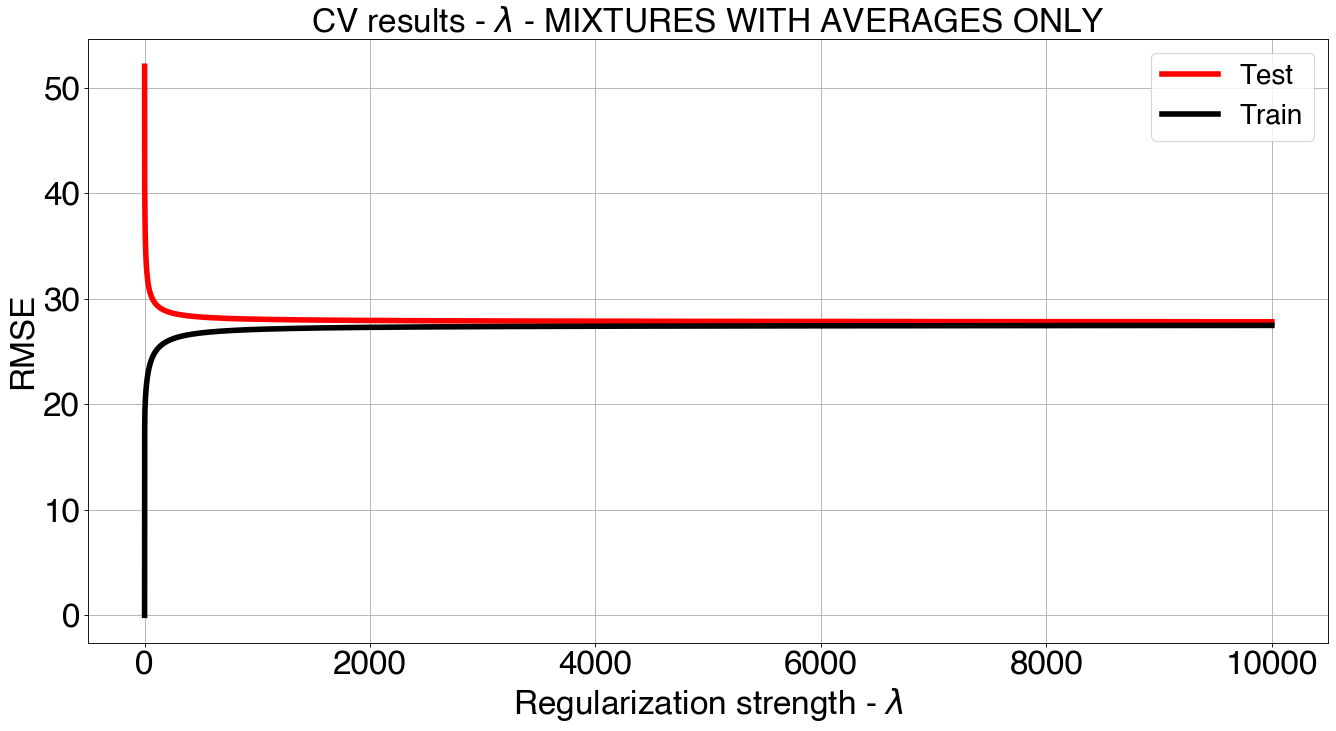
\includegraphics[width=1\linewidth]{../figures/ridge-cv-avg-feat.png}
		\caption{}
		\label{fig:ridge-cv-avg-feat}
	\end{subfigure}
	
	\caption{Cross-validation results for (a) slopes and averages through exposures and (b) only averaged average features through mixtures.}
	\label{fig:ridge-cv-both}
\end{figure}

\begin{figure}[!htb]
	\centering
	
	\begin{subfigure}[t]{0.6\textwidth}
		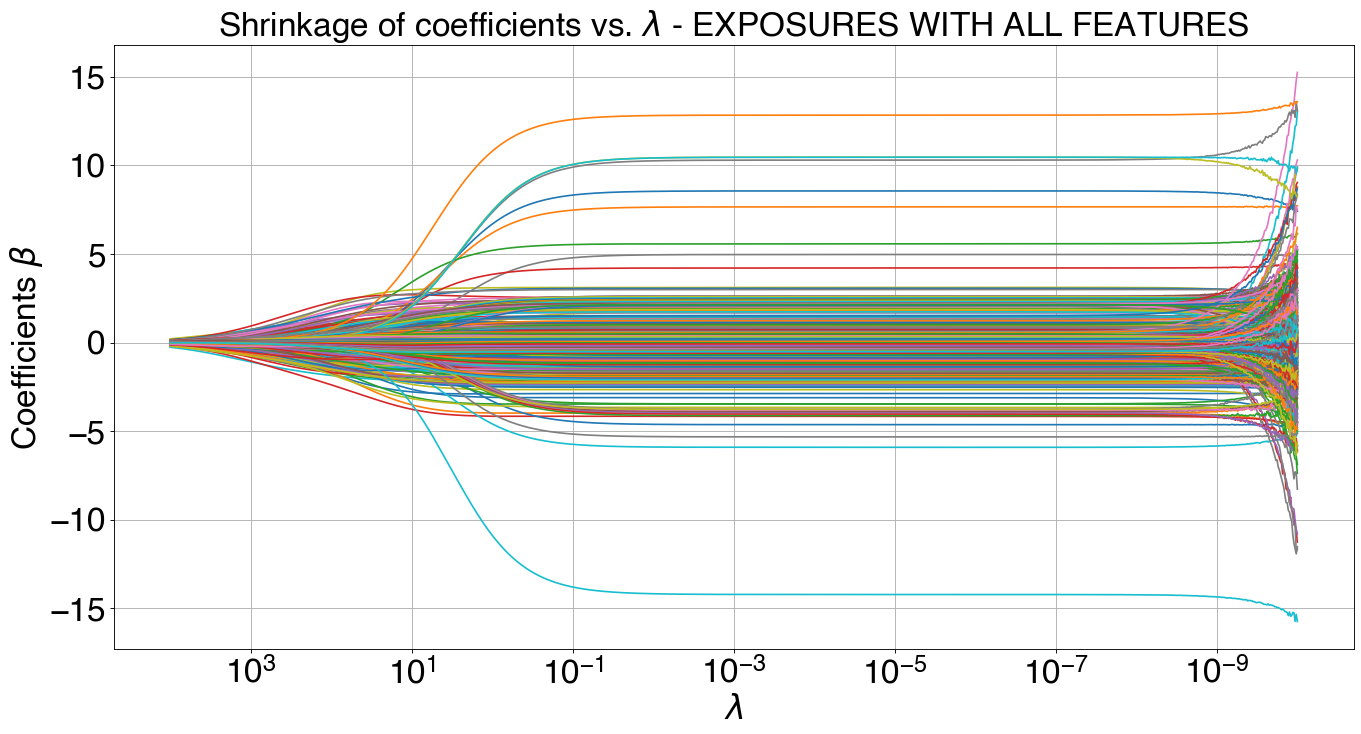
\includegraphics[width=1\linewidth]{../figures/ridge-shrink.png}
		\caption{}
		\label{fig:ridge-shrink} 
	\end{subfigure}
	
	\begin{subfigure}[t]{0.6\textwidth}
		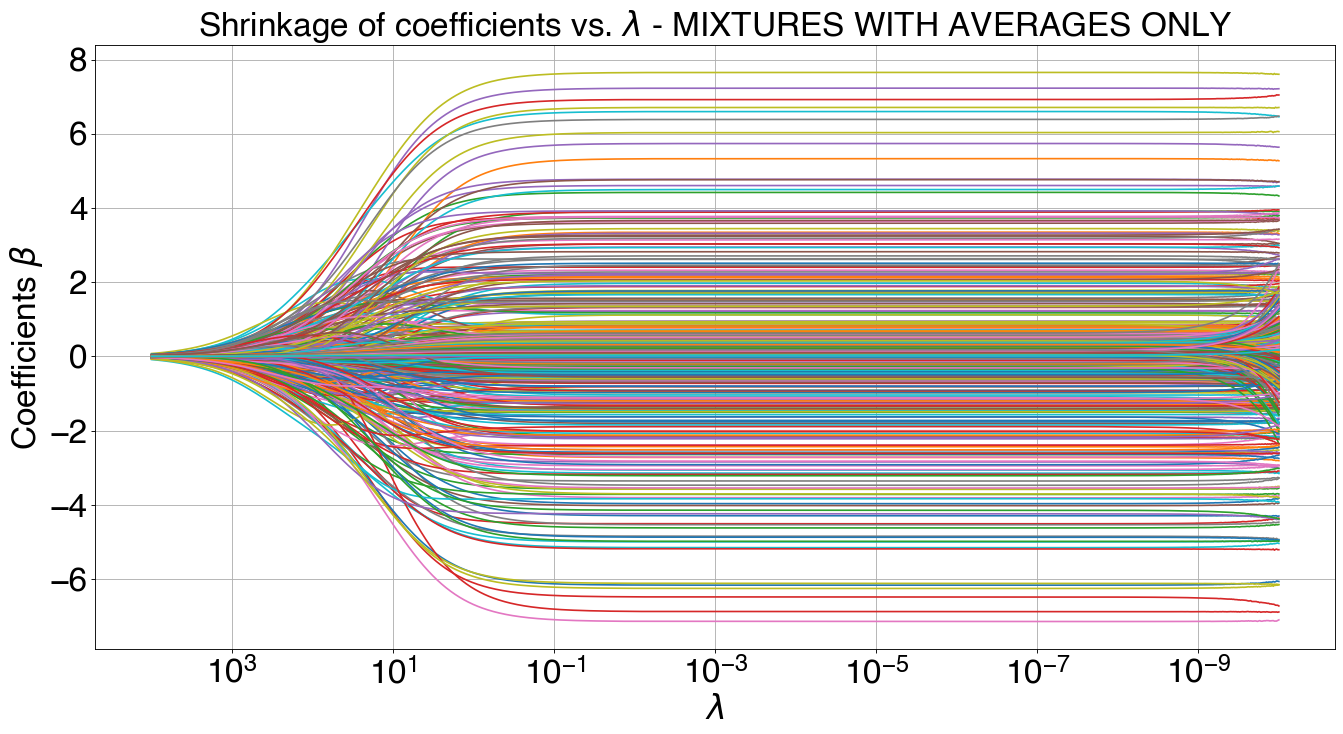
\includegraphics[width=1\linewidth]{../figures/ridge-shrink-avg-feat.png}
		\caption{}
		\label{fig:ridge-shrink-avg-feat}
	\end{subfigure}
	
	\caption{Coefficient shrinkage given $\lambda$ (a) slopes and averages through exposures and (b) only averaged average features through mixtures. Each line corresponds to a coefficient/feature}

	\label{fig:ridge-shrink-both}
\end{figure}

\clearpage
Finally, after the choice of $\lambda = 10000$ (from a grid ranging from $10^{-10}$ to $10^4$), the actual vs. predicted plot is presented in Figure~\ref{fig:ridge-actual-vs-pred-both}. Results here, one more time, seem to be centered around the concentration mean of approximately 31 \acrshort{ppm}.

\begin{figure}[!htb]
	\centering
	
	\begin{subfigure}[t]{1\textwidth}
		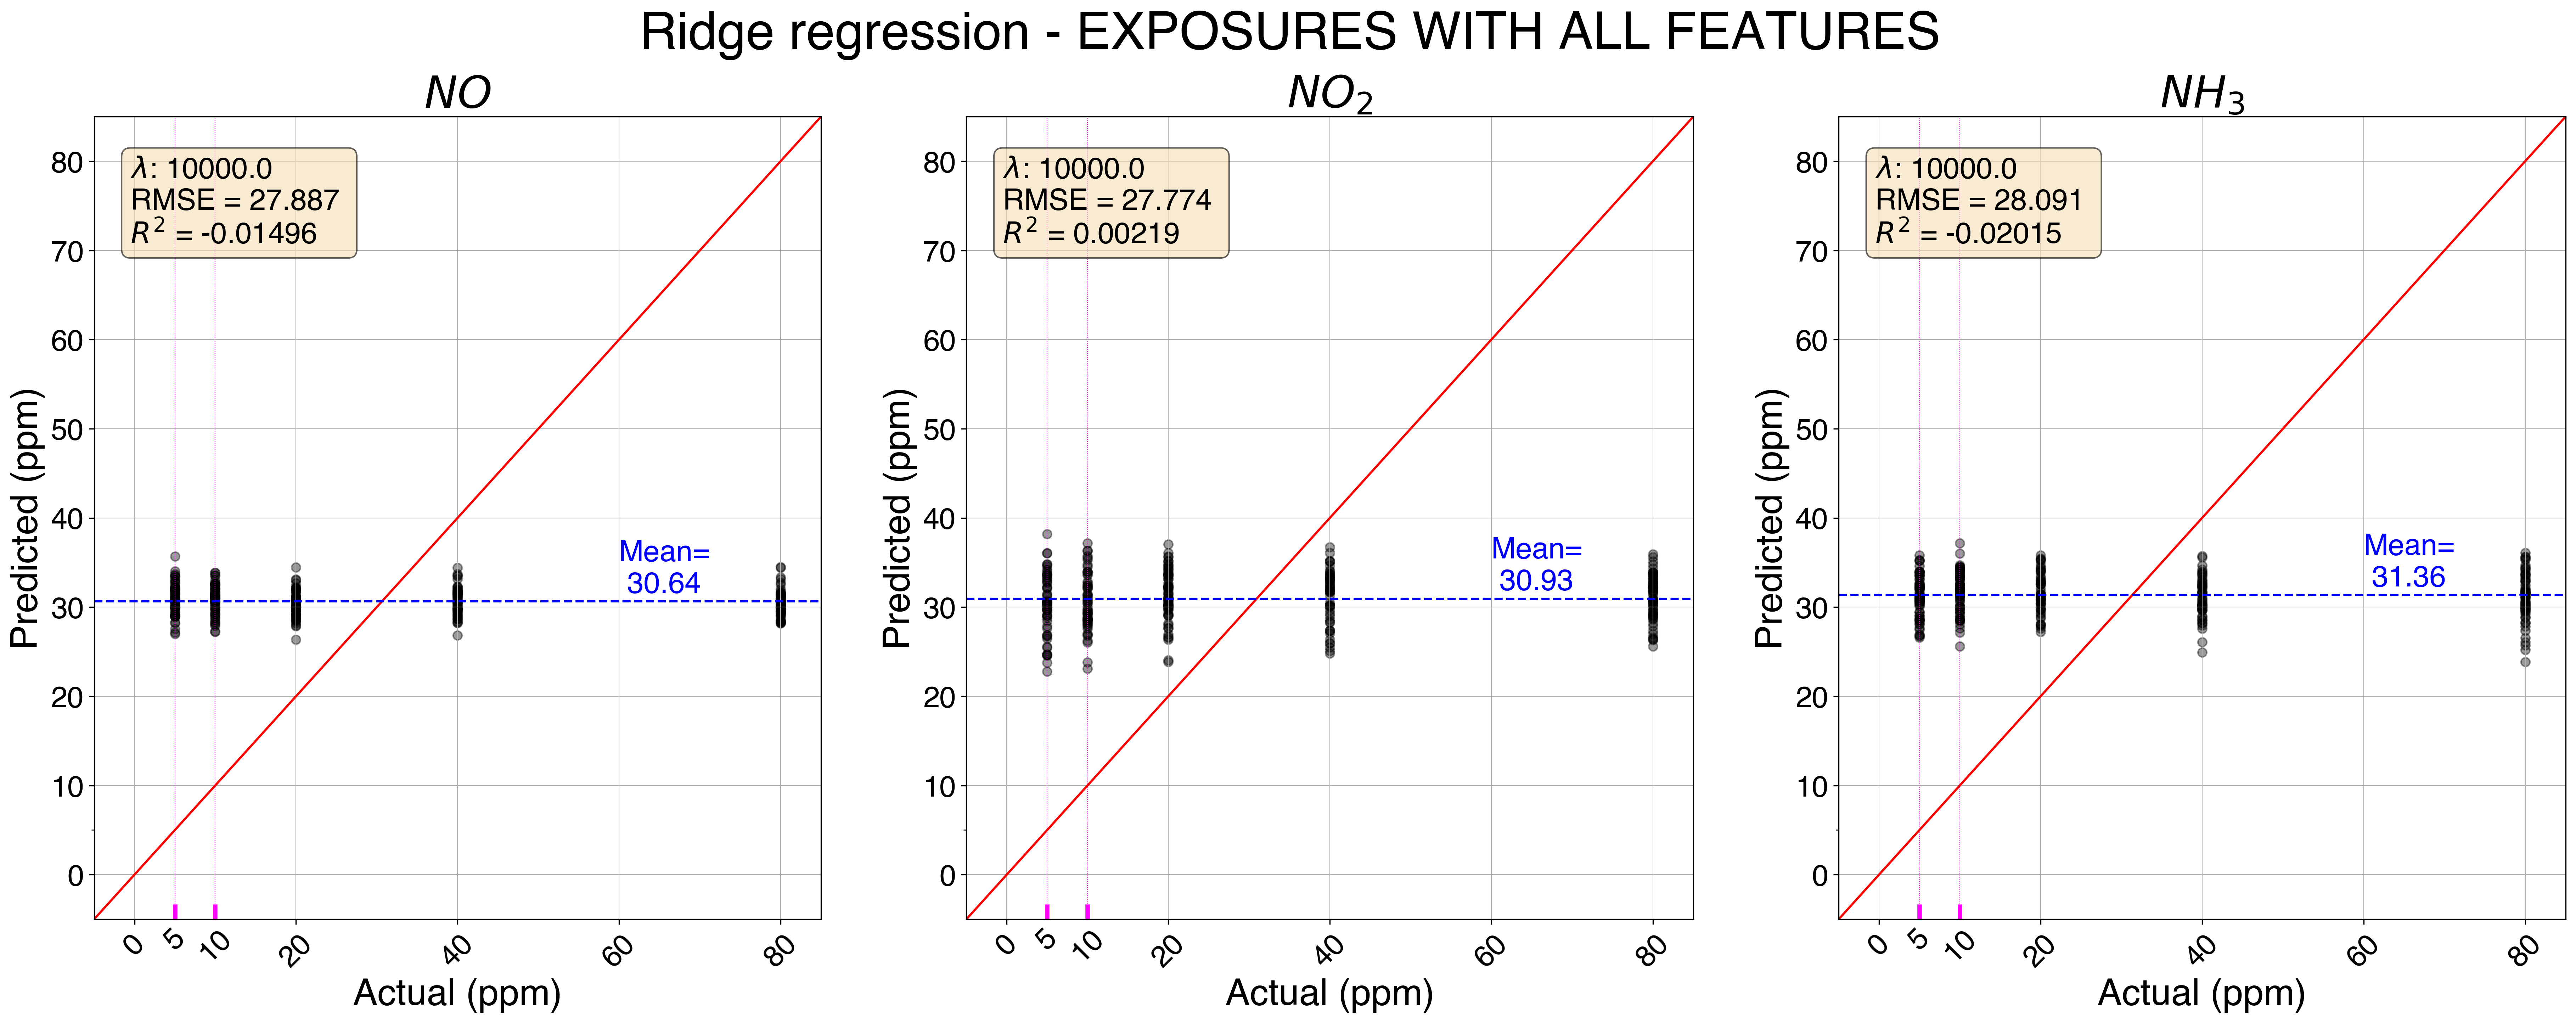
\includegraphics[width=1\linewidth]{../figures/ridge-act-vs-pred.png}
		\caption{}
		\label{fig:ridge-act-vs-pred} 
	\end{subfigure}
	
	\begin{subfigure}[t]{1\textwidth}
		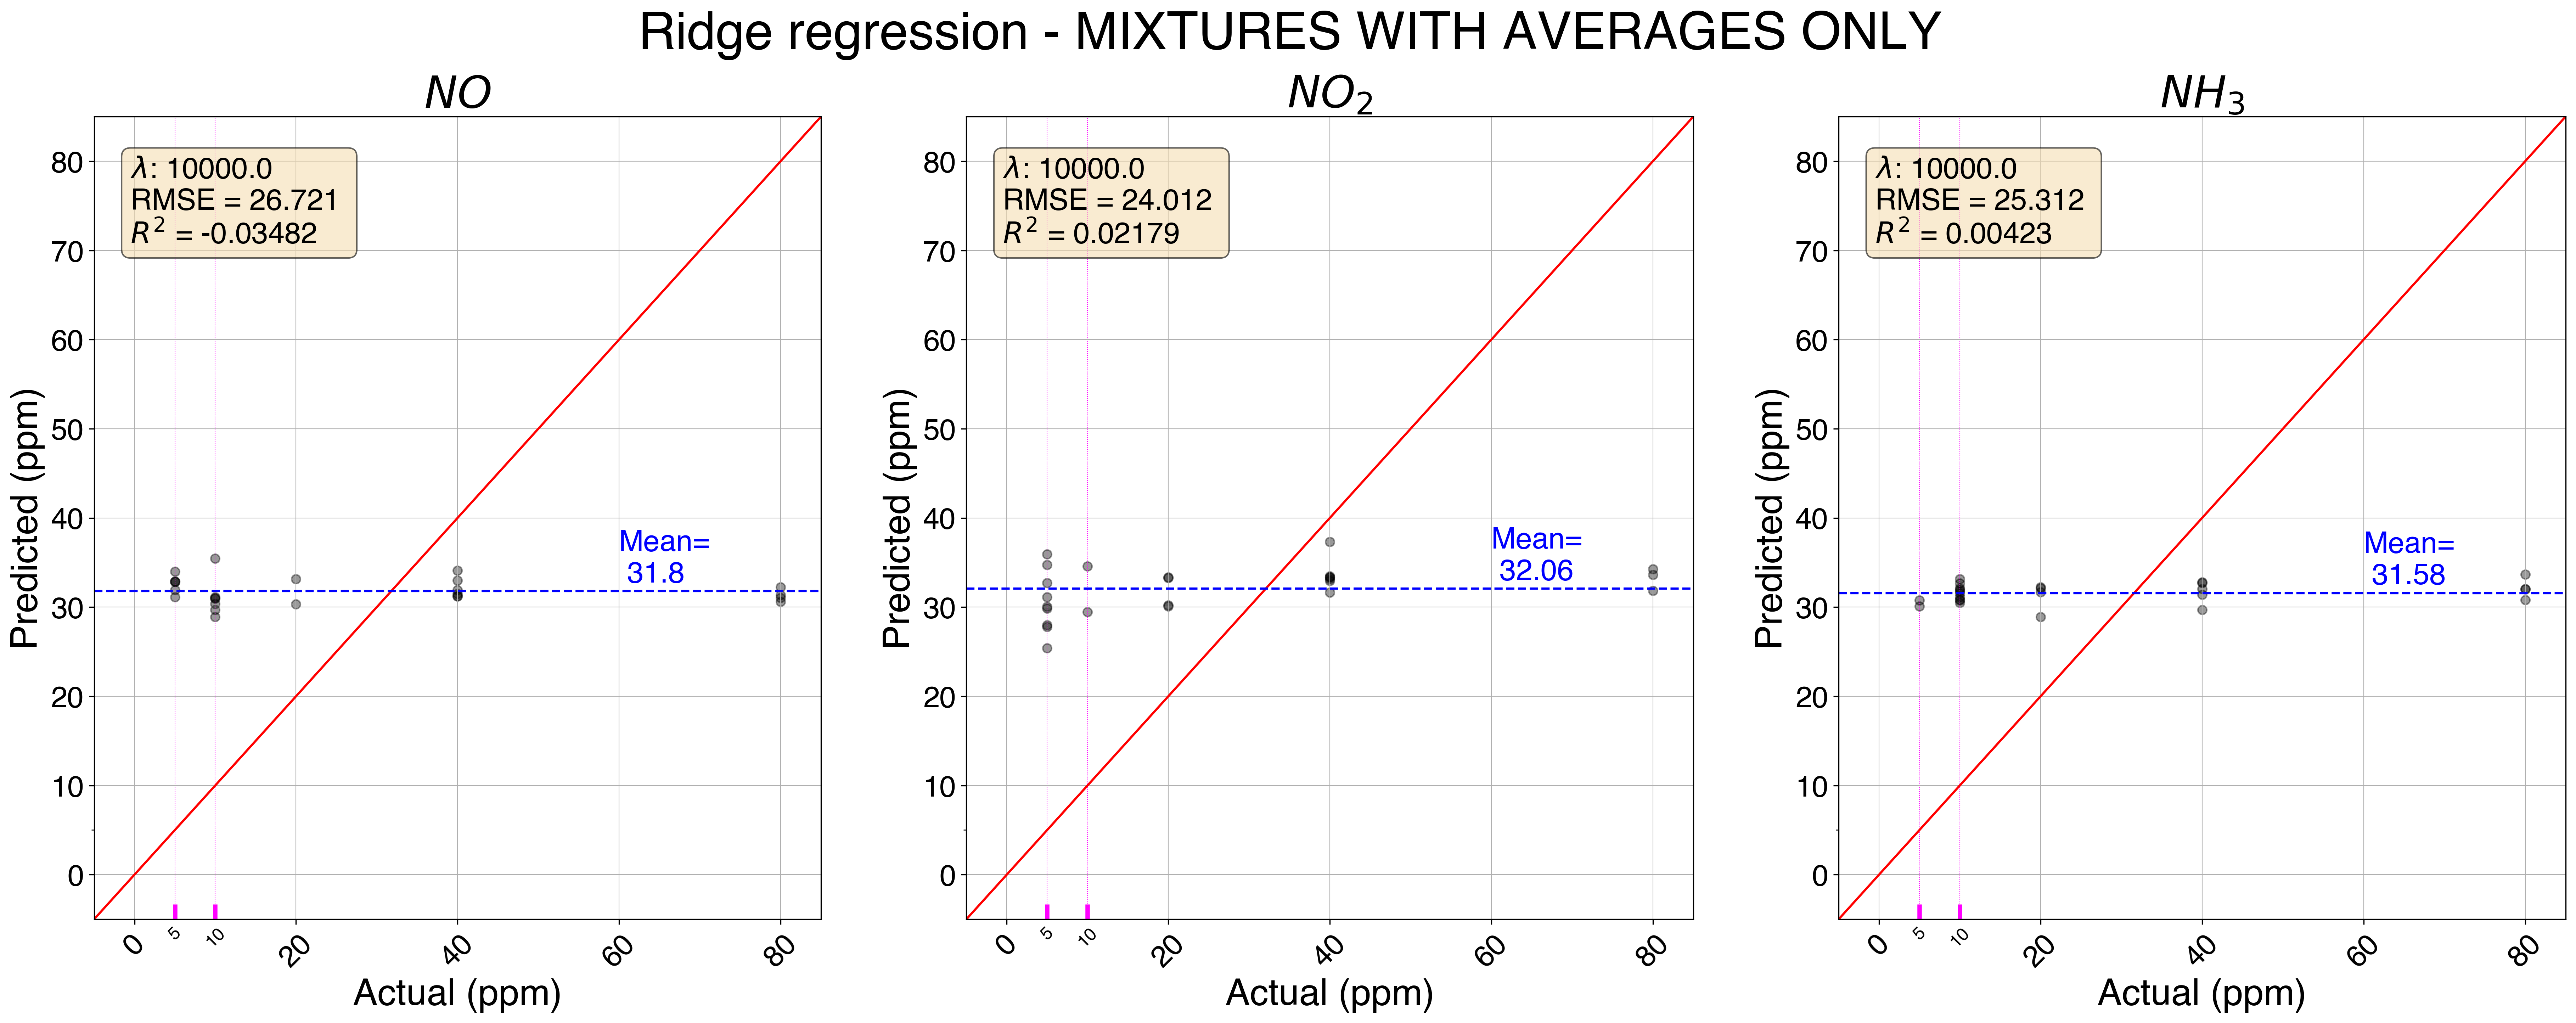
\includegraphics[width=1\linewidth]{../figures/ridge-act-vs-pred-avg-feat.png}
		\caption{}
		\label{fig:ridge-act-vs-pred-avg-feat}
	\end{subfigure}
	
	\caption{Ridge regression predictions for (a) slopes and averages through exposures and (b) only averaged average features through mixtures.}
	\label{fig:ridge-actual-vs-pred-both}
\end{figure}




